\documentclass[11pt]{beamer}

\usepackage{booktabs}
\usepackage{multirow}
\usepackage{subfigure} 

%\def\argmax{\operatornamewithlimits{arg\,max}}
%\def\argmin{\operatornamewithlimits{arg\,min}}

\def\O{{\ensuremath{\mathcal{O}}}}
\def\M{{\ensuremath{\mathcal{M}}}}
\def\t{{\ensuremath{\theta}}}
\def\tt{{\ensuremath{\tilde{\theta}}}}
\def\R{\rm I\!R}

\usepackage{algorithmic}

%%%%%%% Referencing
\newcommand\reffig[1]{Figure \ref{fig:#1}}
\newcommand\refsec[1]{Section \ref{sec:#1}}

%%%%%%% Comments
\newcommand\sw[1]{\emph{\textcolor{red}{#1}}}

%%%%%%% Stuff
\newcommand{\theHalgorithm}{\arabic{algorithm}}
\newcommand{\xbest}{\mathbf{\vx}^{+}}
\newcommand{\xstar}{\mathbf{\vx}^{*}}
\newcommand{\ystar}{\mathbf{\vy}^{*}}
\DeclareMathOperator*{\argmin}{arg\,min}
\DeclareMathOperator*{\argmax}{arg\,max}
\DeclareMathOperator*{\T}{^\intercal}
\newcommand{\norm}[1]{\left\lVert#1\right\rVert}
\newcommand*{\thead}[1]{\mlticolumn{1}{c}{#1}}
\newcommand{\pluseq}{\mathrel{+}=}

%%%%%%% Kamil's expectations and vars.
\newcommand{\ex}[1]{{\mathbb E}\left[ #1 \right]}
\newcommand{\exc}[2]{{\mathbb E}\left[ #1 \,\middle \vert\, #2 \right]}
\newcommand{\exs}[2]{{\mathbb E_{#1}}\left[ #2 \right]}
\newcommand{\vars}[2]{{\mathbb V_{#1}}\left[ #2 \right]}
\newcommand{\excs}[3]{{\mathbb E_{#1}}\left[ #2 \,\middle \vert\, #3 \right]}

\newcommand{\bld}[1]{\emph{\textcolor{red}{#1}}}
\newcommand{\fd}[1]{\textcolor{gray}{#1}}

\definecolor{lightyellow}{rgb}{1,0.98,0.71}
\newcommand{\paper}[1]{\begin{center}\colorbox{lightyellow}{%
\begin{minipage}{0.9\textwidth}\scriptsize
#1\end{minipage}}\end{center}}

\renewcommand{\algorithmicrequire}{\textbf{Input:}}
\renewcommand{\algorithmicensure}{\textbf{Return:}}
\renewcommand{\algorithmiccomment}[1]{// \textit{#1}}

\mode<presentation>
{
  \usetheme{Boadilla}
  \usecolortheme{dolphin}
  \usefonttheme{structurebold}
%  \setbeamercovered{transparent}
  \setbeamertemplate{navigation symbols}{}
}

%\pgfdeclareimage[height=0.5cm]{institution-logo}{uva_logo}
%\logo{\pgfuseimage{institution-logo}}

\title[Factored VFs for Cooperative MARL]{Factored Value Functions for Cooperative Multi-Agent Reinforcement Learning}
\author[Shimon Whiteson (Oxford)]{Shimon Whiteson \\ Dept.\ of Computer Science \\ University of Oxford \\ \ \\ joint work with Jakob Foerster, Gregory Farquhar, Anuj Mahajan,\\ Tabish Rashid, Mikayel Samvelyan, Christian Schroeder de Witt,\\
Nantas Nardelli, Tim Rudner, Chia-Man Hung, and Phil Torr}
\date{\today}

\begin{document}

\frame{\titlepage}

\frame{
\frametitle{Single-Agent Paradigm}
%%%%%%%%%%%%%%%%%

\begin{center}
  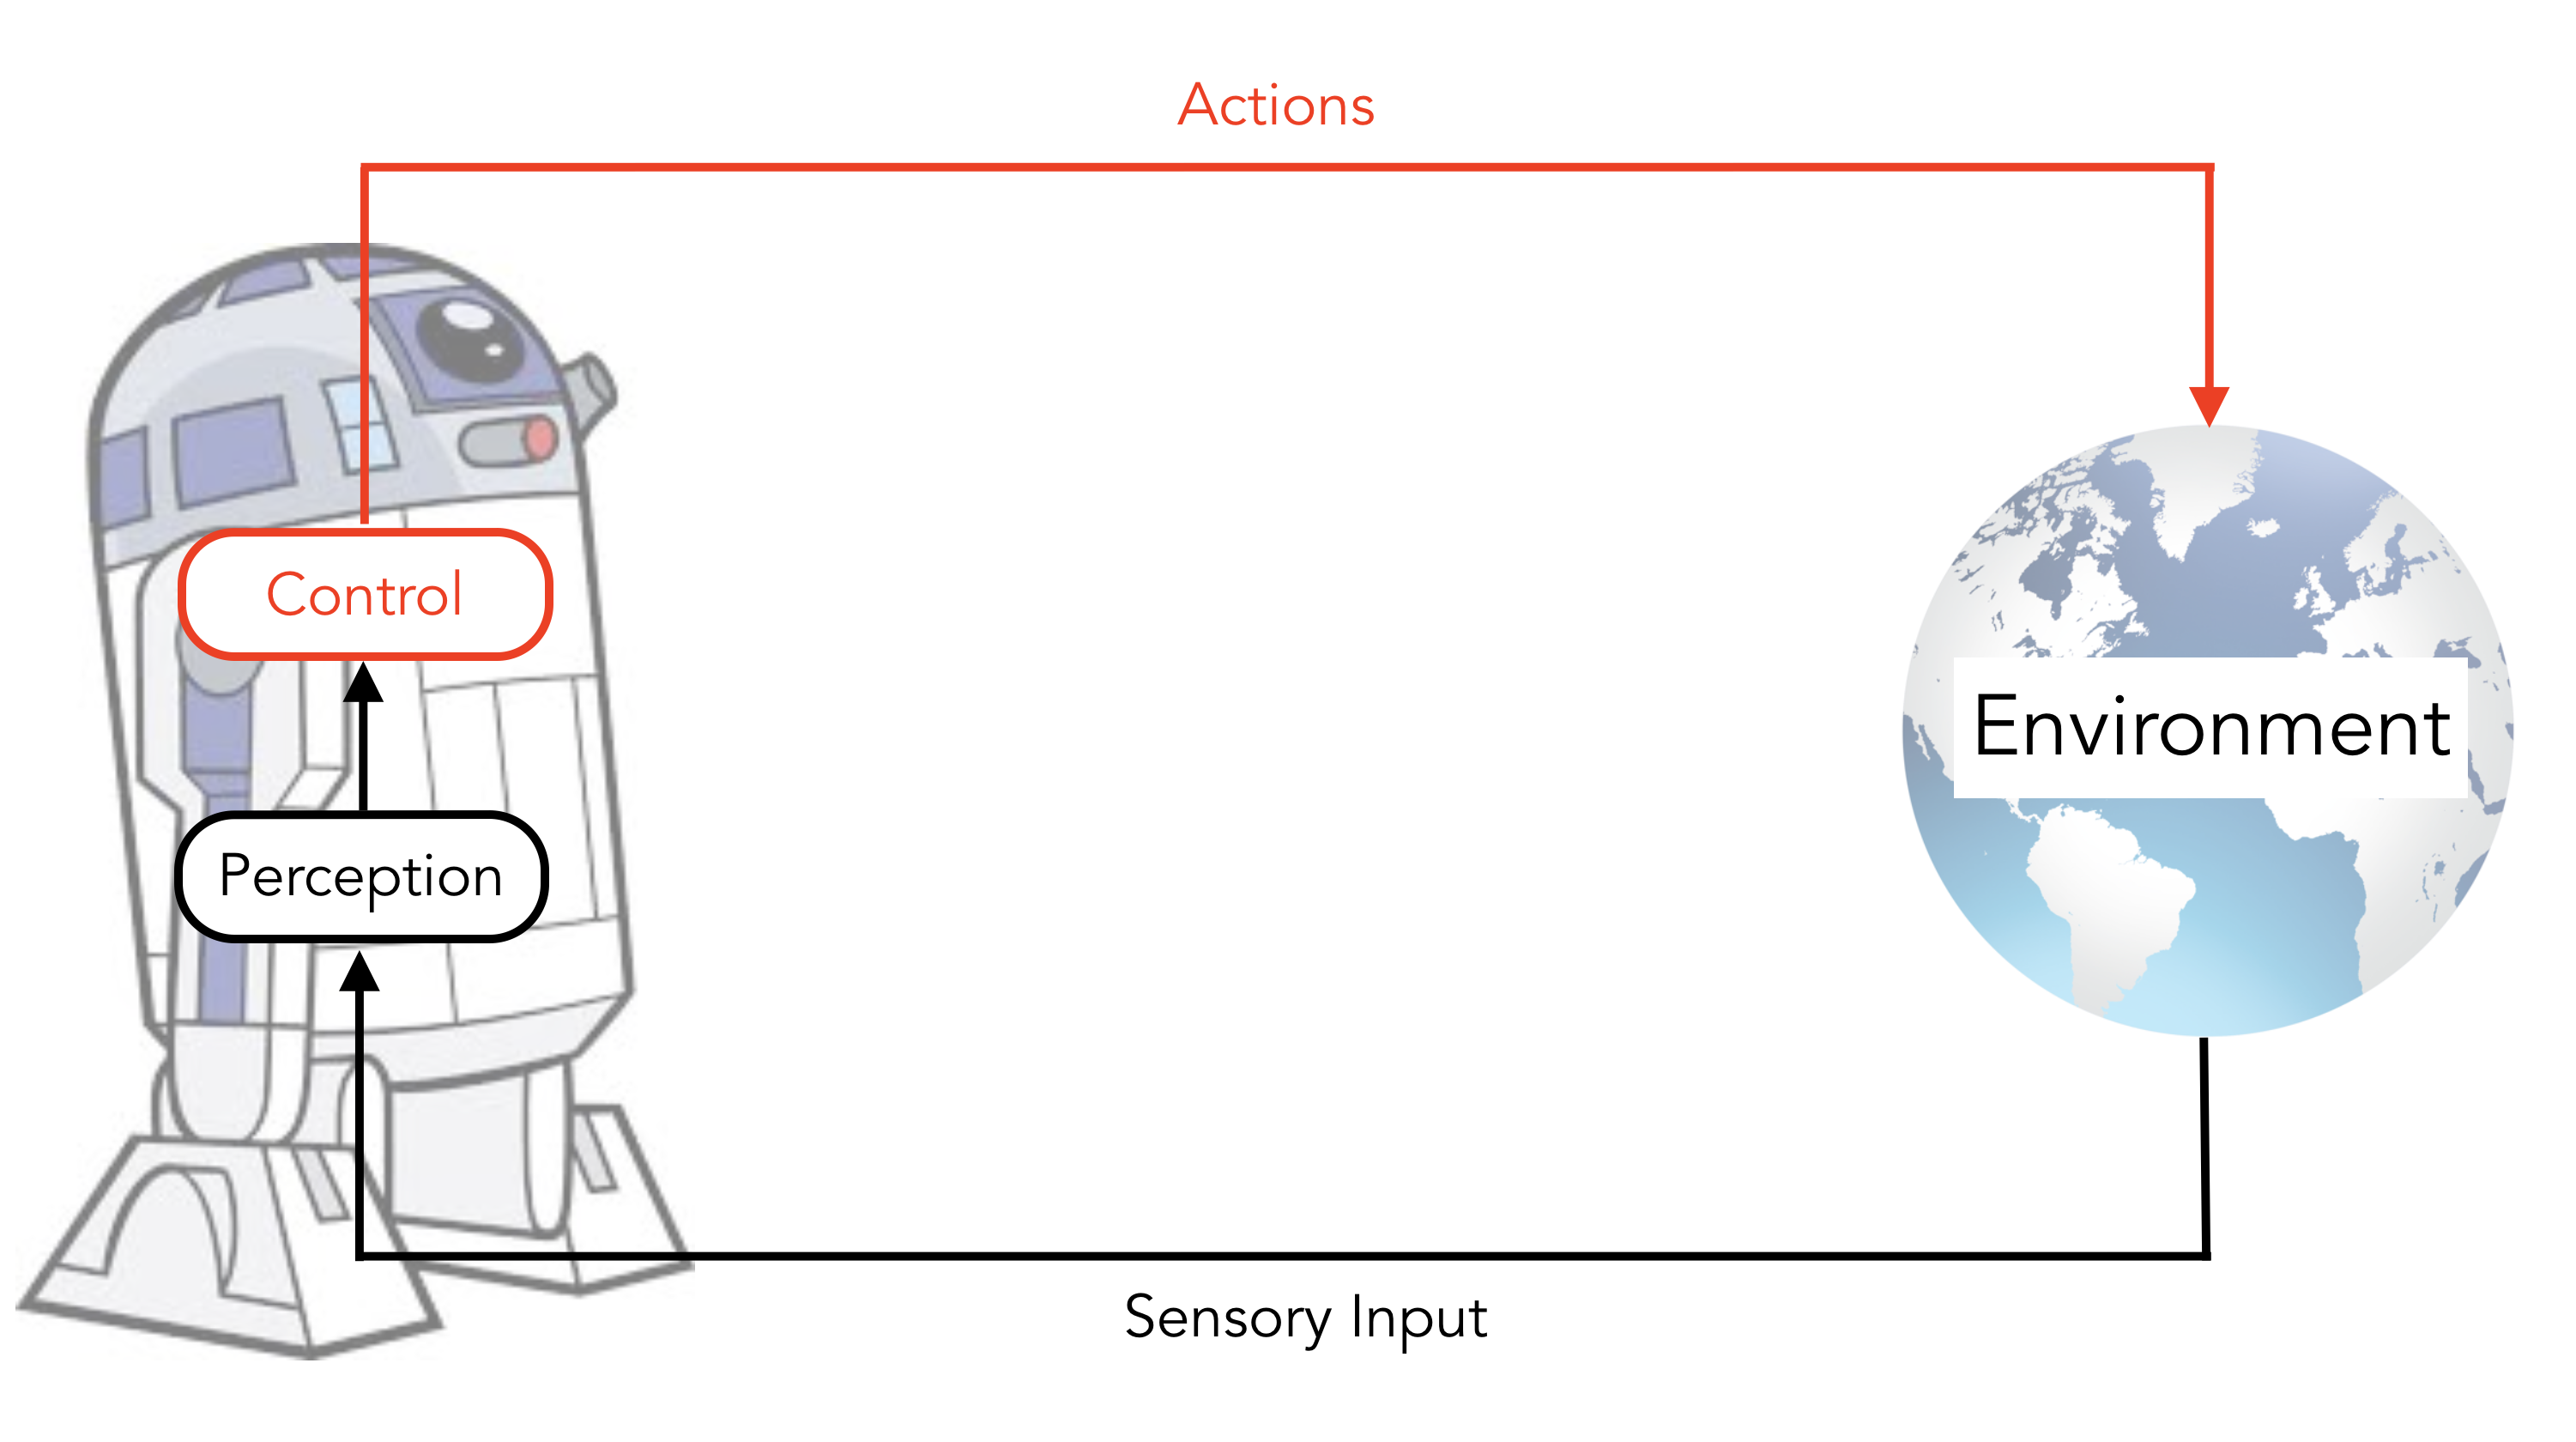
\includegraphics[scale = 0.2]{rl}
\end{center} 

}

\frame{
\frametitle{Multi-Agent Paradigm}
%%%%%%%%%%%%%%%%%

\begin{center}
  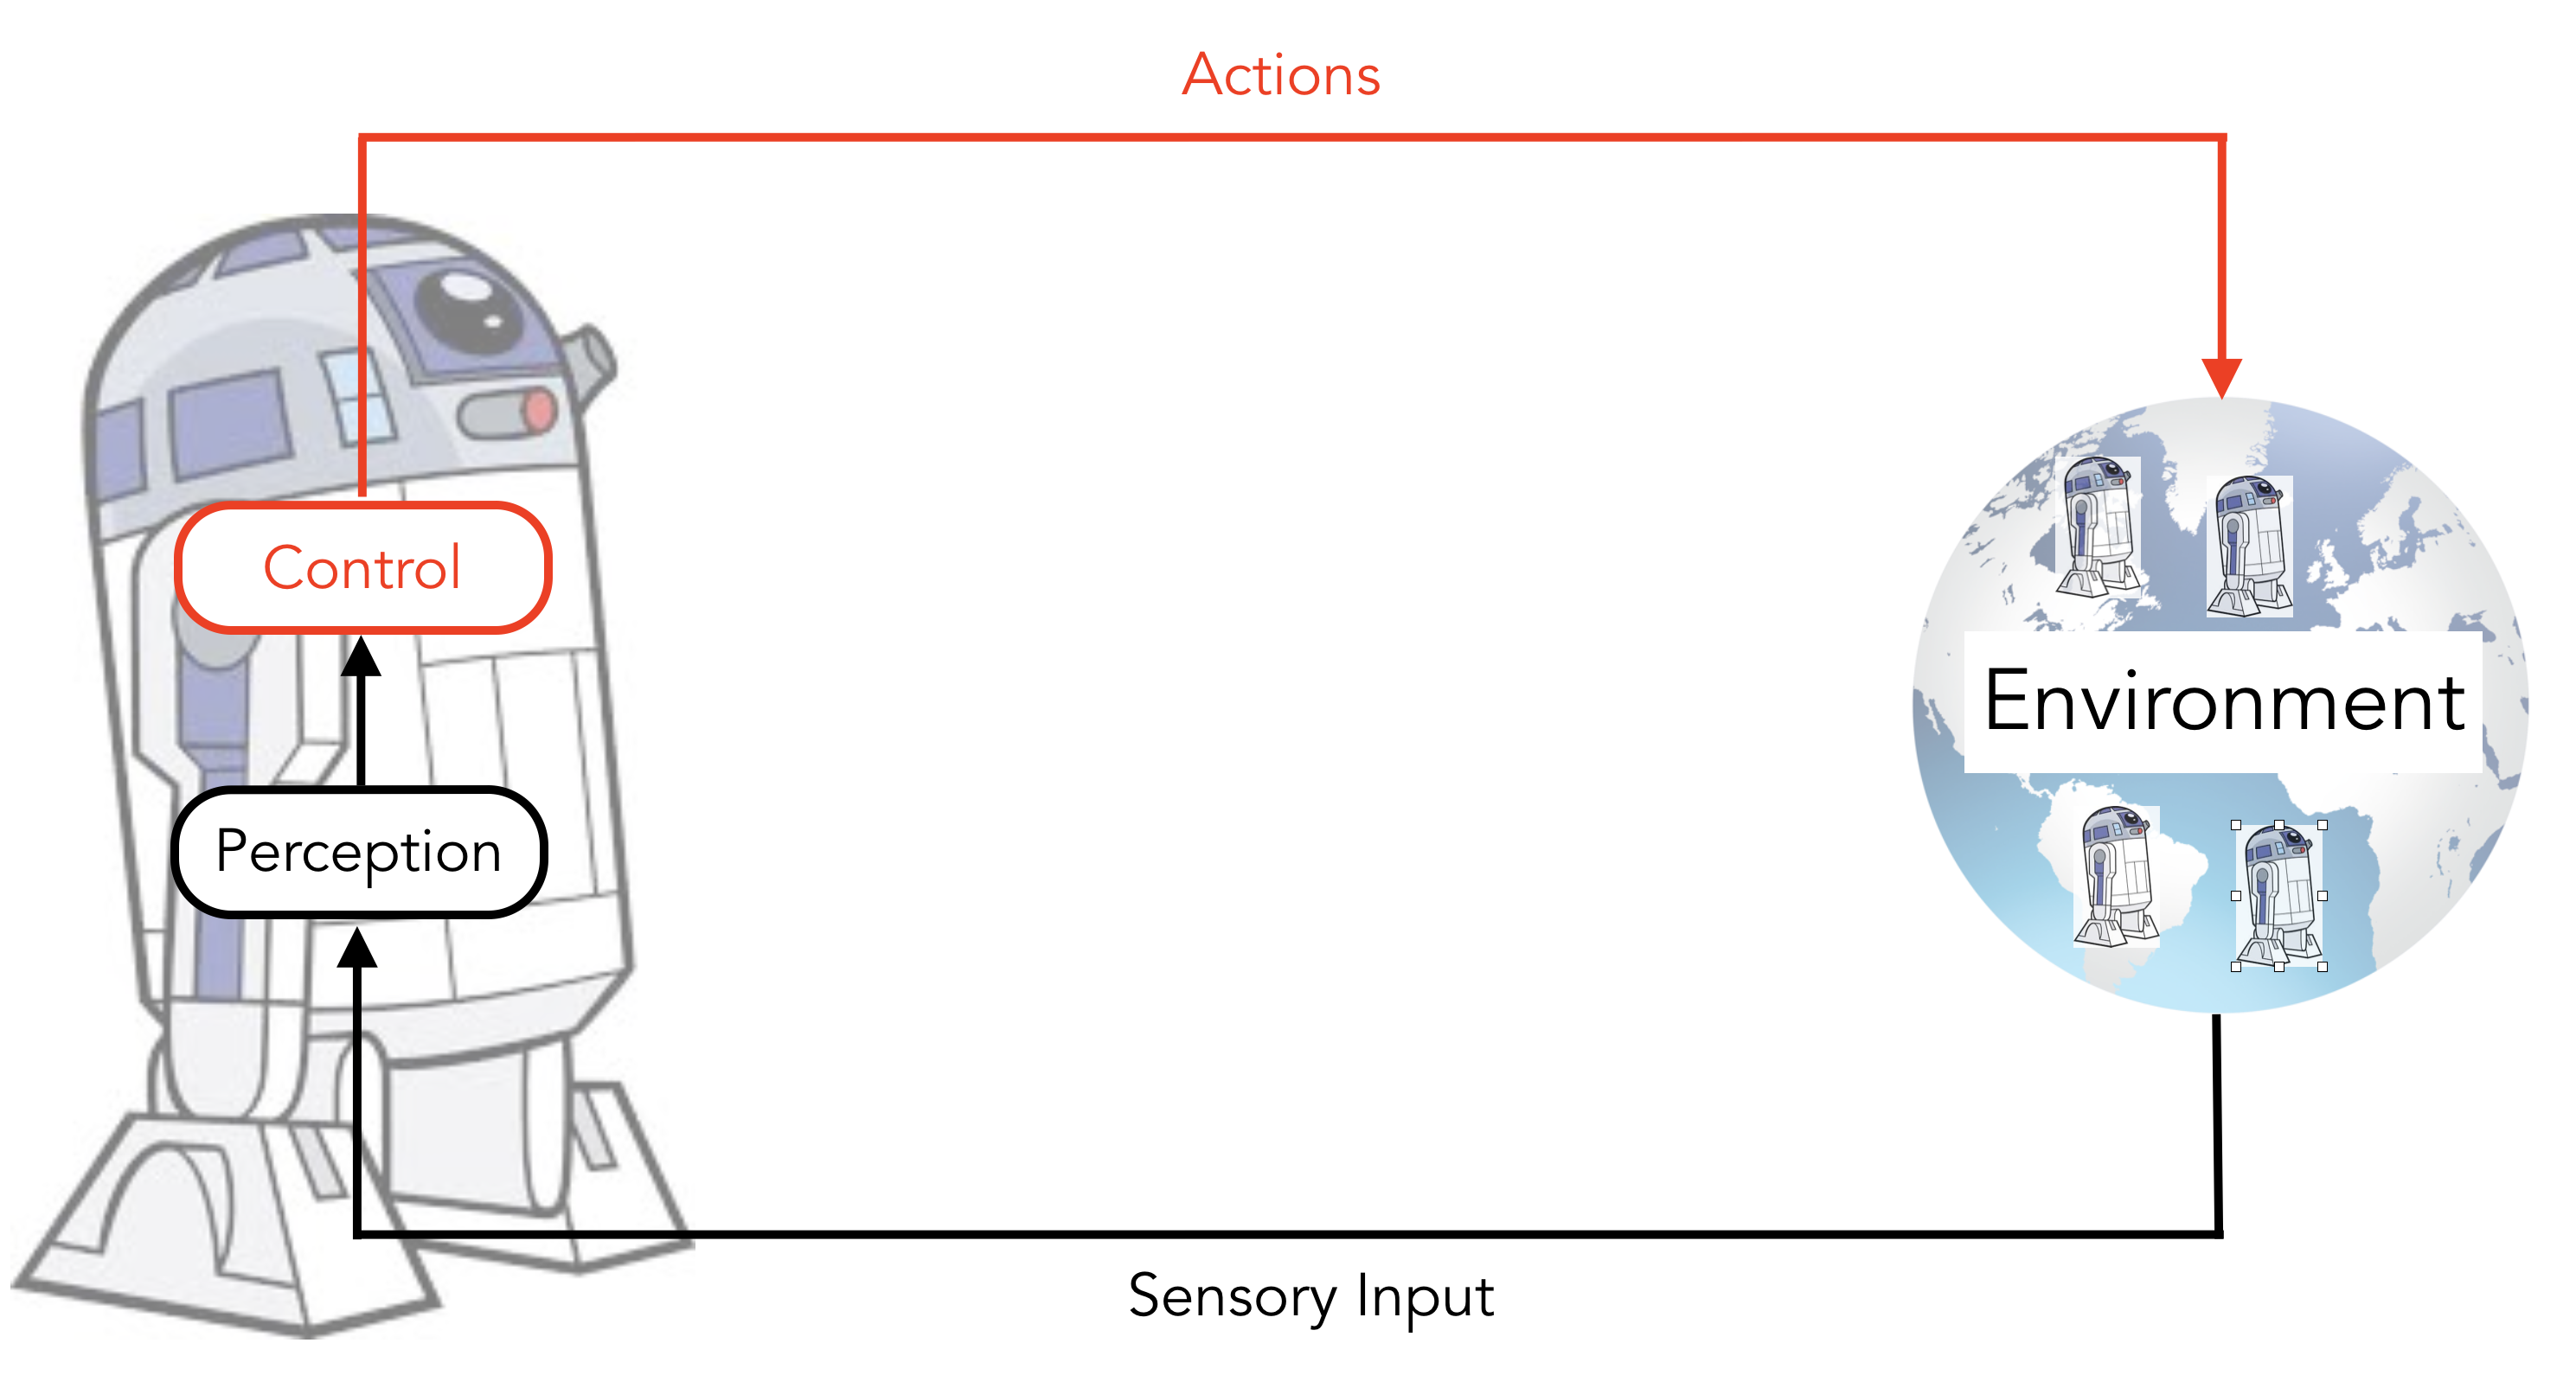
\includegraphics[scale = 0.2]{marl}
\end{center} 

}

\frame{
\frametitle{Multi-Agent Systems are Everywhere}
%%%%%%%%%%%%%%%%%

\begin{center}
%  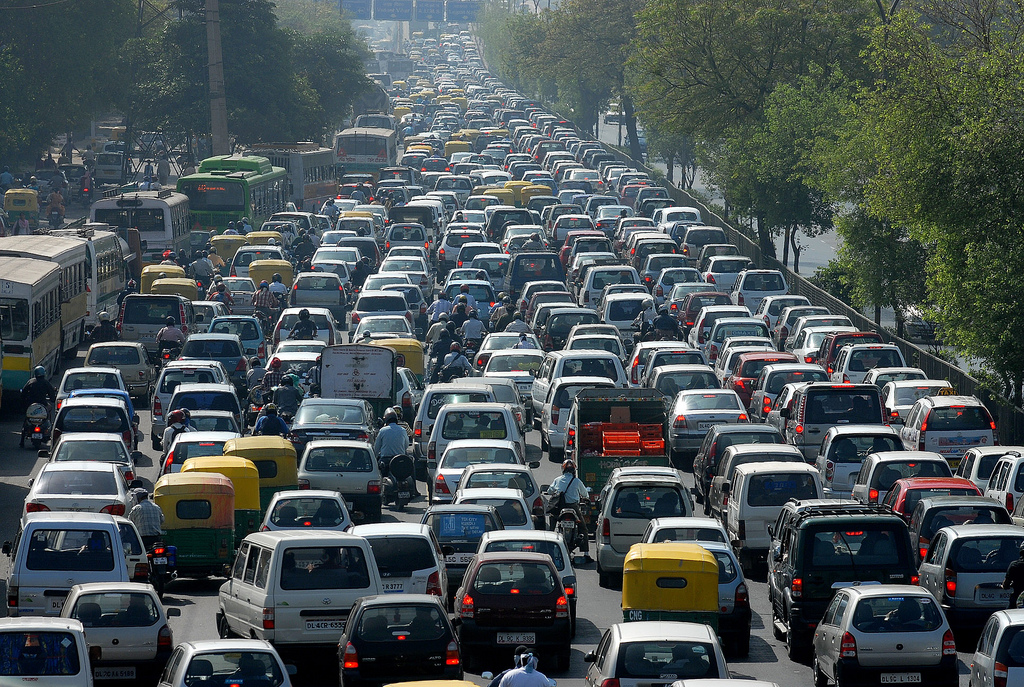
\includegraphics[scale = 0.4]{traffic-jam}
%  \hspace{1cm}
%  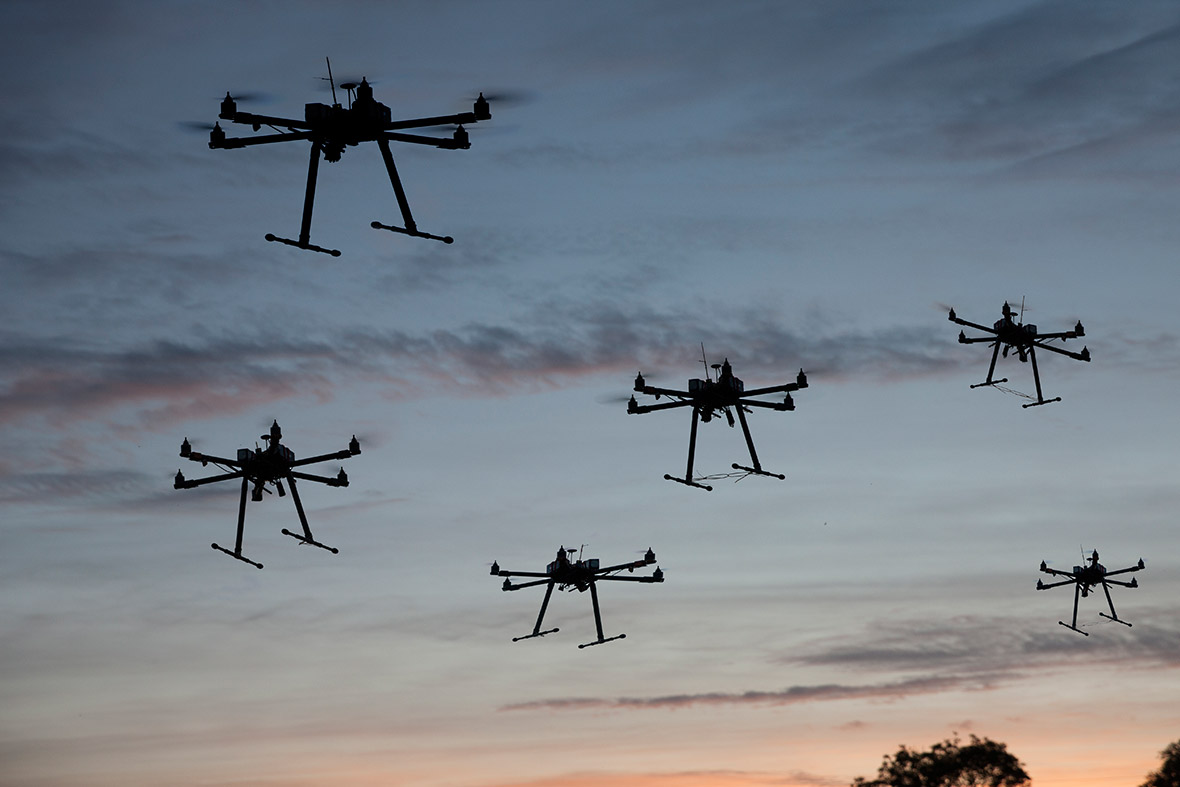
\includegraphics[scale = 0.125]{many-drones}
  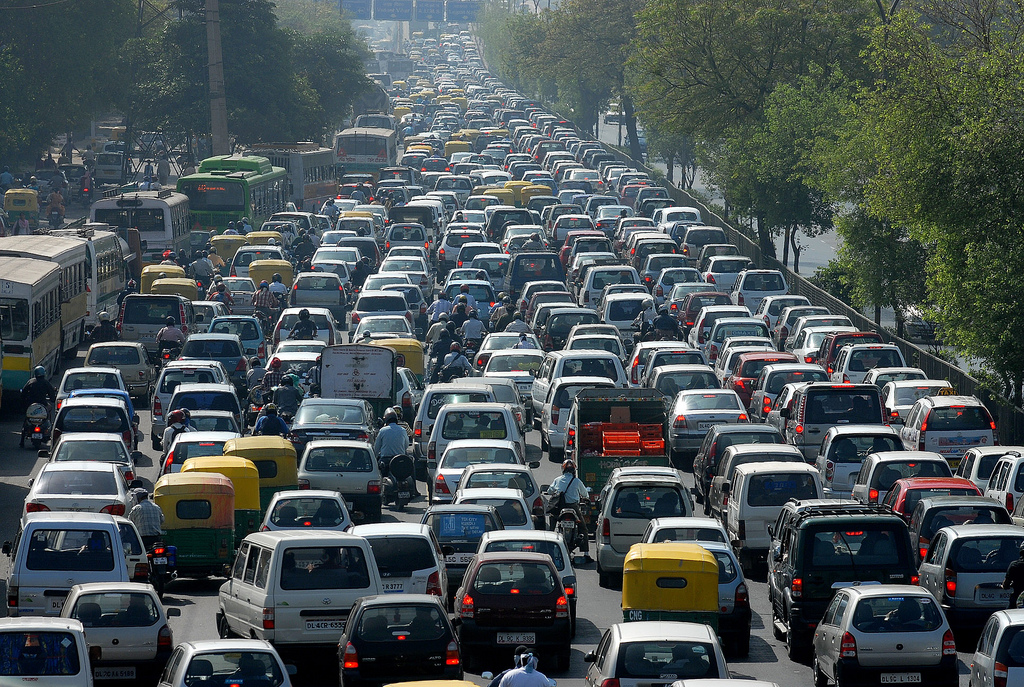
\includegraphics[width=0.45\linewidth]{traffic-jam}
  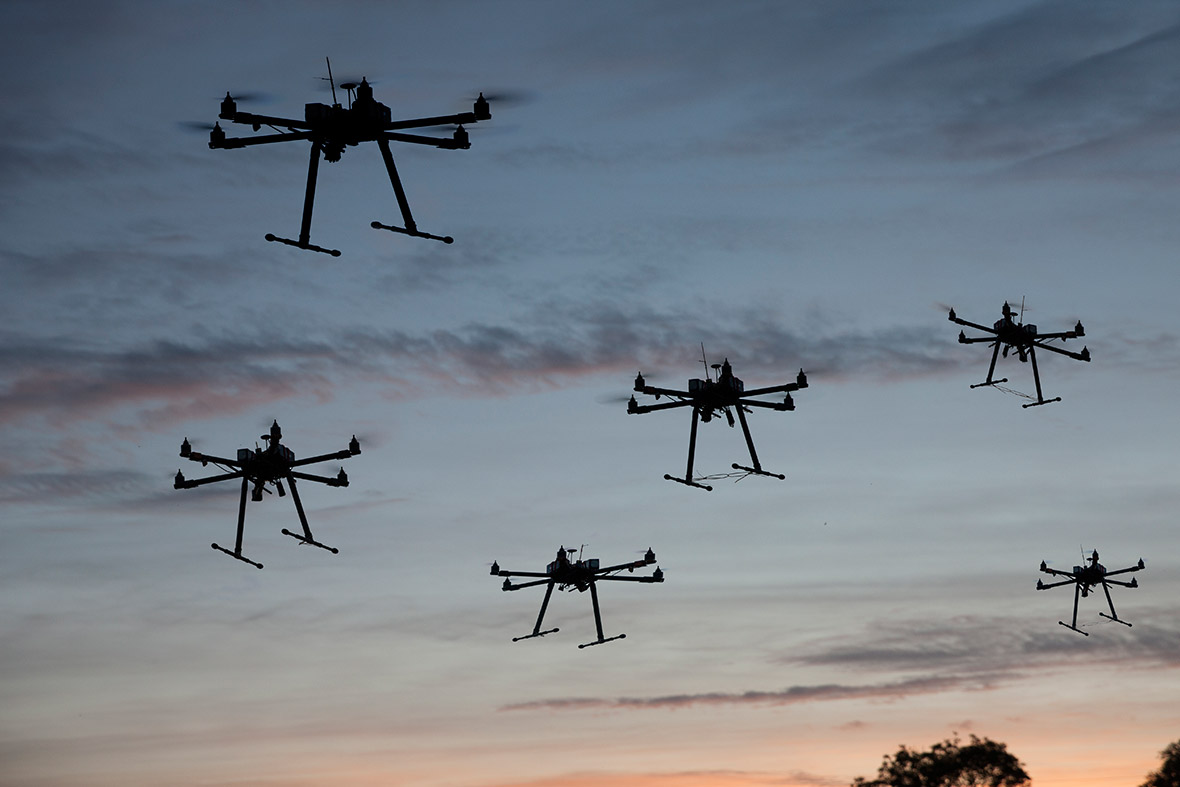
\includegraphics[width=0.45\linewidth]{many-drones}\\
  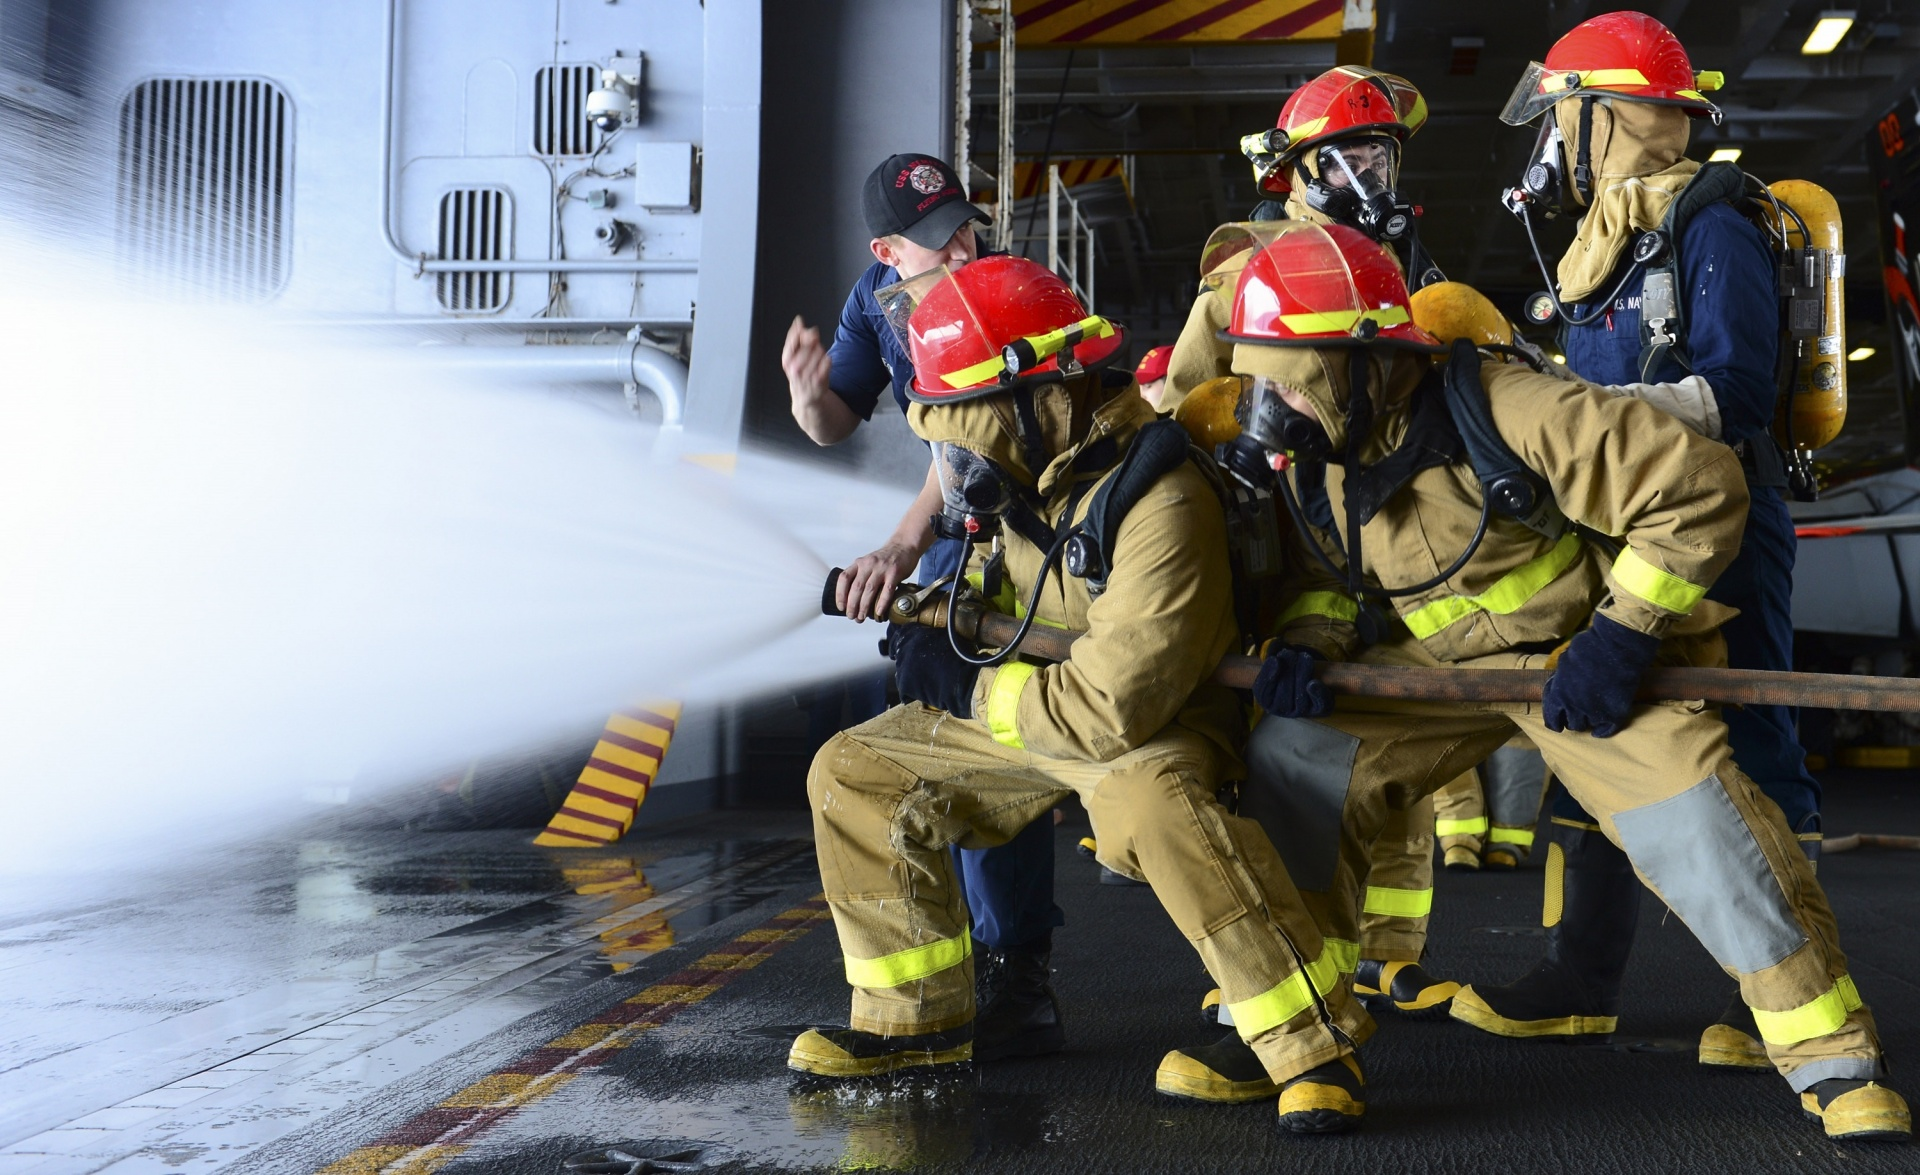
\includegraphics[width=0.45\linewidth]{firemen}
  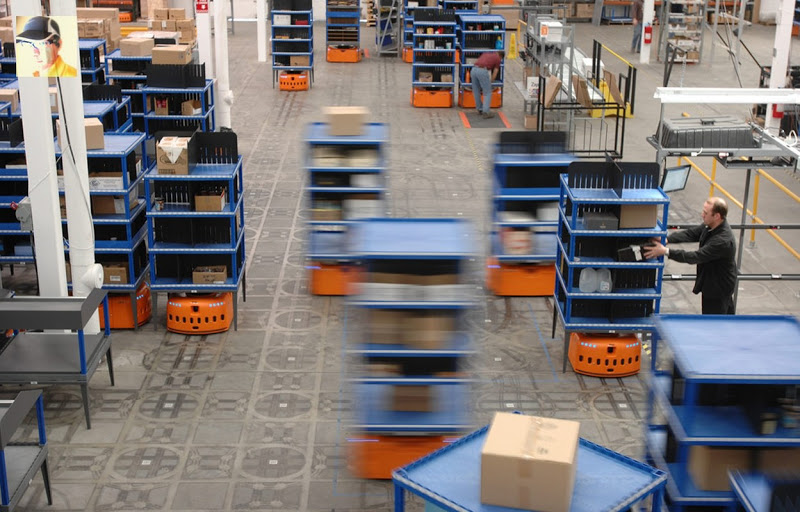
\includegraphics[width=0.45\linewidth]{kiva}    
\end{center} 

}

\frame{
\frametitle{Types of Multi-Agent Systems}
%%%%%%%%%%%%%%%%%

\begin{itemize}
	\item \sw{Cooperative:} 
		\begin{itemize}
			\item Shared team reward
			\item Coordination problem
		\end{itemize}
	\vspace{5mm}
	\item \sw{Competitive:}
		\begin{itemize}
			\item Zero-sum games
			\item Individual opposing rewards
			\item Minimax equilibria
		\end{itemize}
	\vspace{5mm}		
	\item \sw{Mixed:}
		\begin{itemize}
			\item General-sum games
			\item Nash equilibria
			\item What is the question? [Shoham et al.\ 2007]
		\end{itemize}
\end{itemize}
}

\frame{
\frametitle{Coordination Problems are Everywhere}
%%%%%%%%%%%%%%%%%

\begin{center}
%  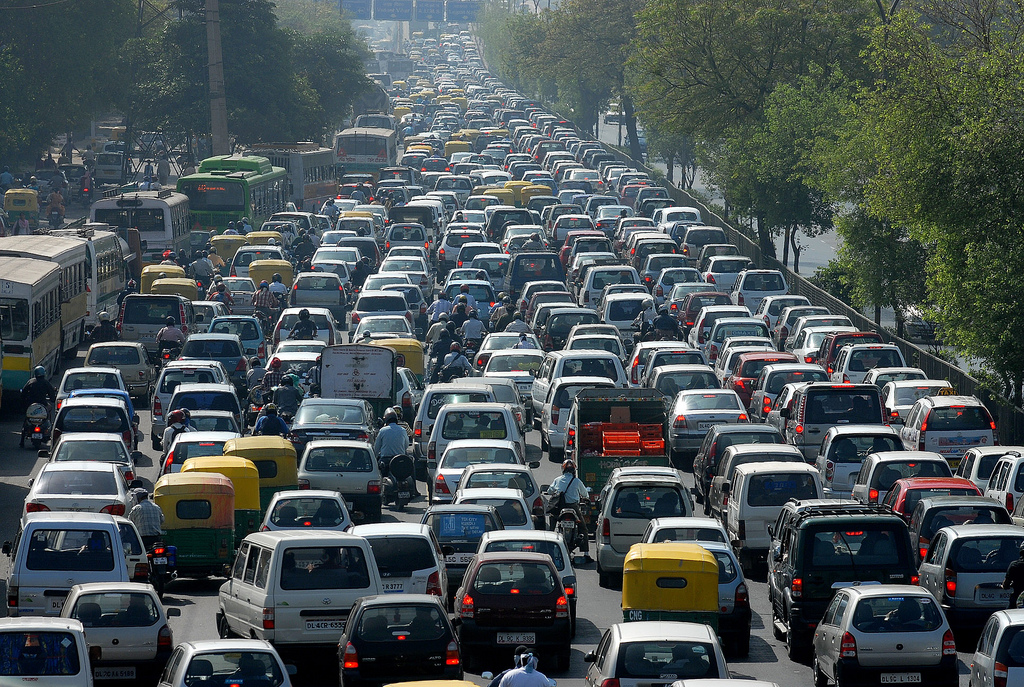
\includegraphics[scale = 0.4]{traffic-jam}
%  \hspace{1cm}
%  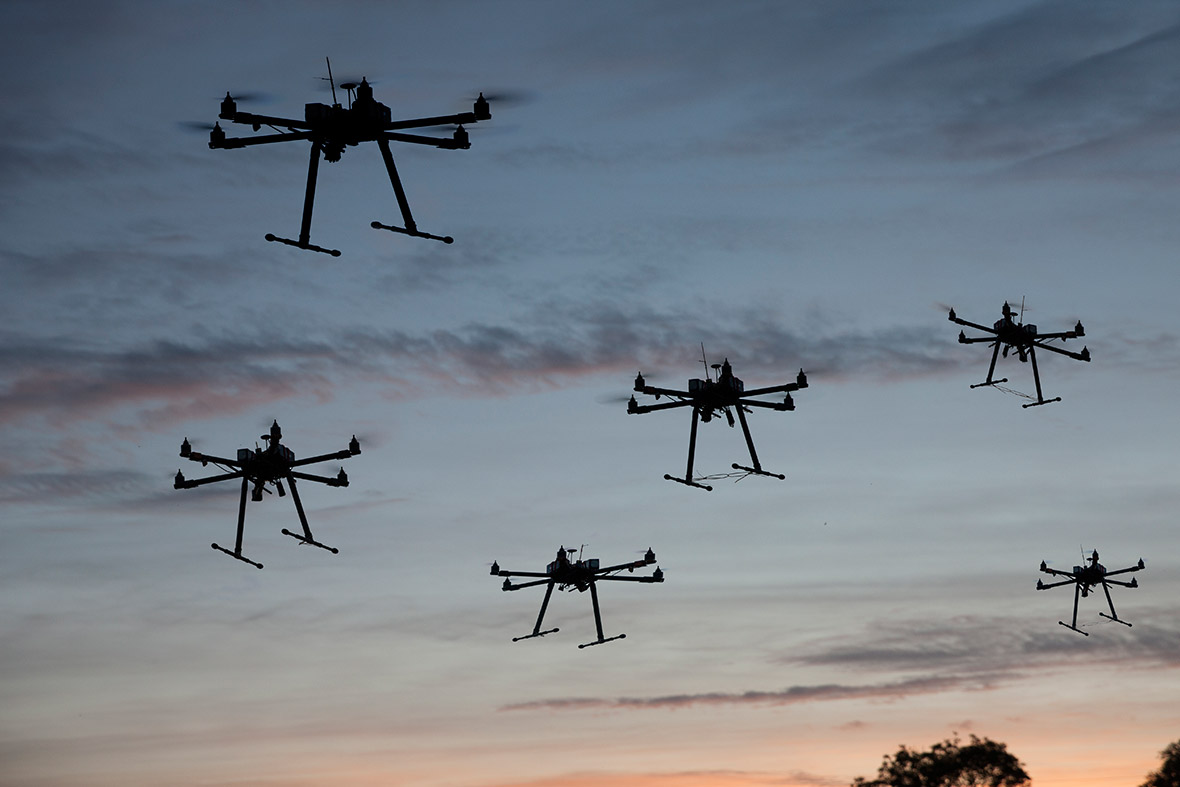
\includegraphics[scale = 0.125]{many-drones}
  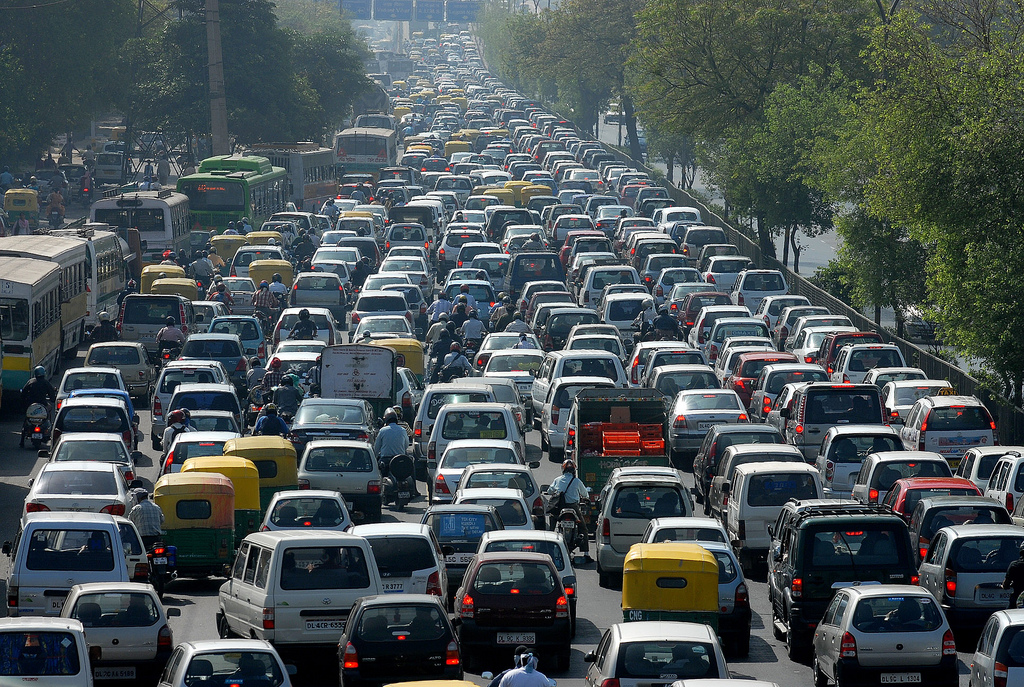
\includegraphics[width=0.45\linewidth]{traffic-jam}
  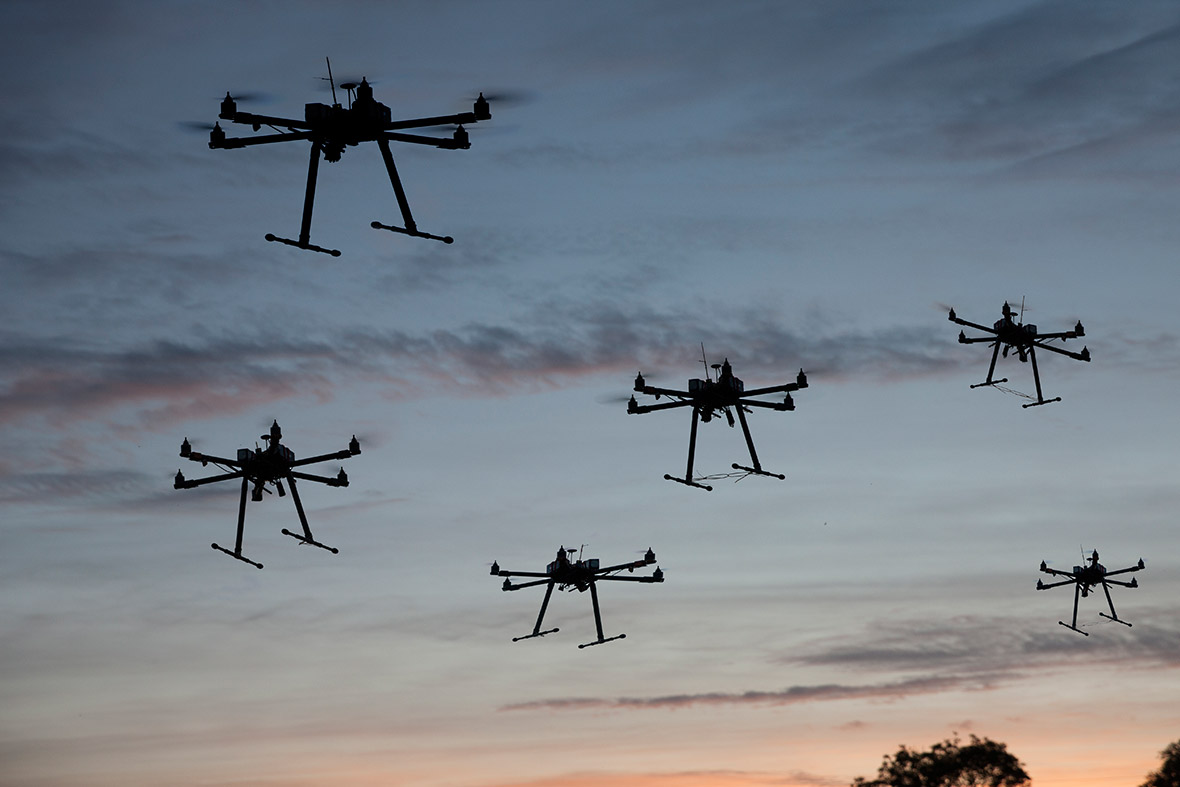
\includegraphics[width=0.45\linewidth]{many-drones}\\
  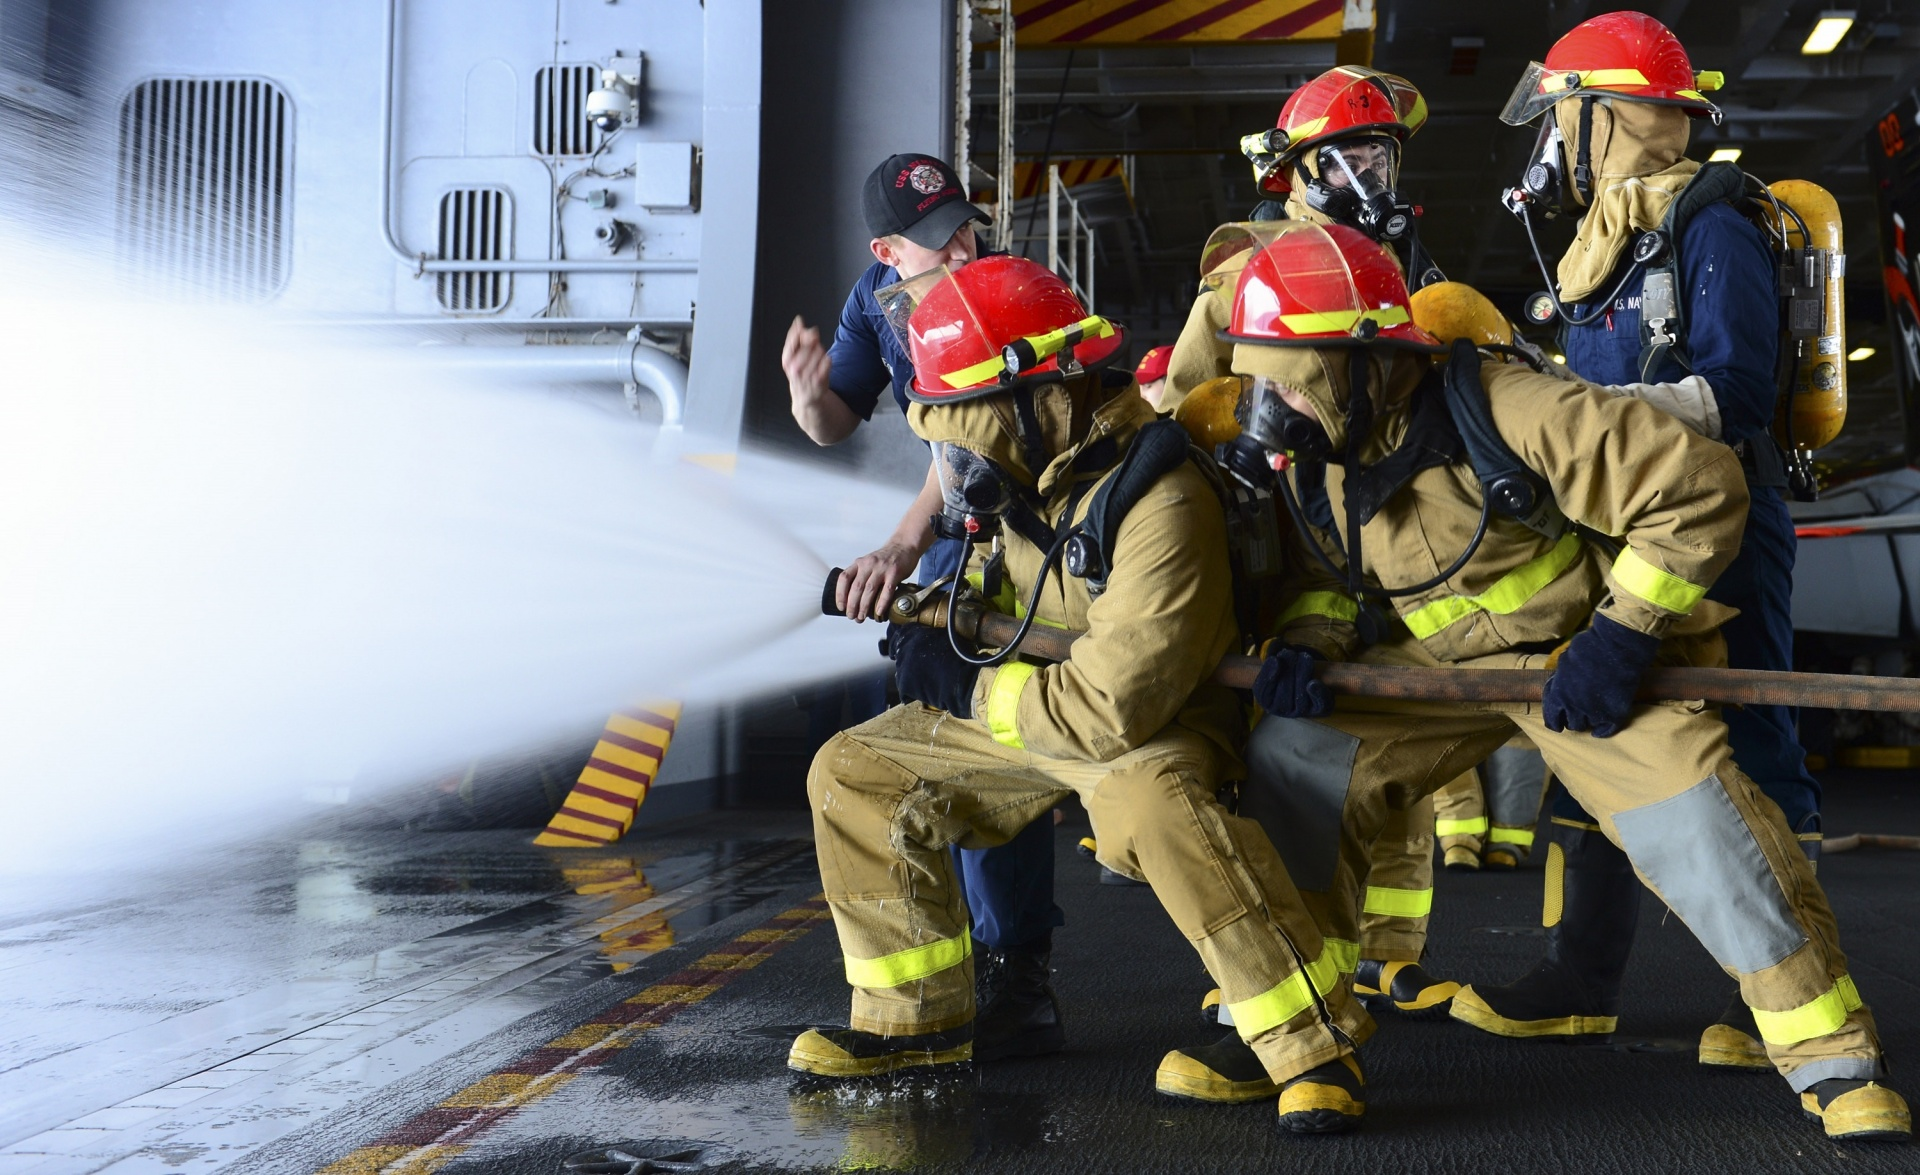
\includegraphics[width=0.45\linewidth]{firemen}
  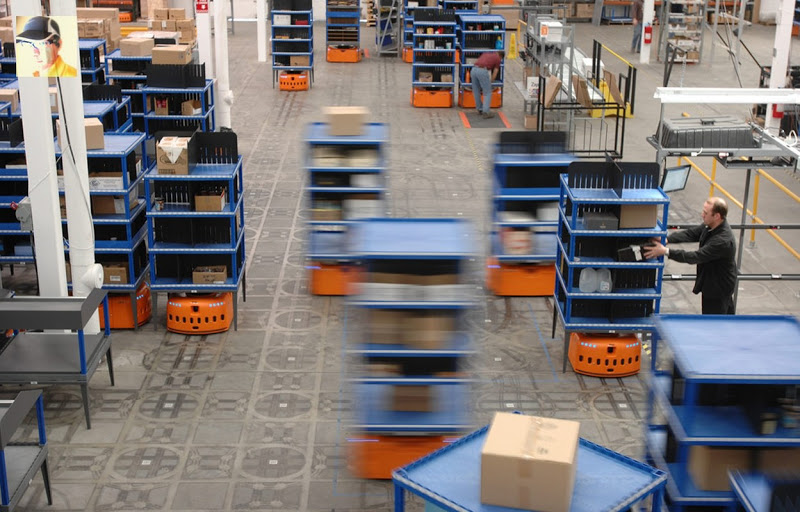
\includegraphics[width=0.45\linewidth]{kiva}    
\end{center} 

}

%\frame{
%\frametitle{Update rules}
%%%%%%%%%%%%%%%%%%
%
%\begin{itemize}
%
%	\item \sw{Temporal difference} (TD) update rule:
%		\begin{equation*}
%		V(s_t) \leftarrow V(s_t) + \alpha[r_t + \gamma V(s_{t+1}) - V(s_t)]
%		\end{equation*}
%	\item \sw{Sarsa} update rule:
%		\begin{equation*}
%		Q(s_t,u_t) \leftarrow Q(s_t,u_t) + \alpha[r_t + \gamma Q(s_{t+1},u_{t+1}) - Q(s_t,u_t)]		
%		\end{equation*}
%	\item \sw{Q-learning} update rule:
%	\begin{equation*}
%	 	Q(s_t,u_t) \leftarrow Q(s_t,u_t) + \alpha[r_t + \gamma \max_u Q(s_{t+1},u) - Q(s_t,u_t)]	
%	\end{equation*}
%	\item Act (soft) \sw{greedily} wrt to $Q$-values:
%	\begin{equation*}
%		u_t = \argmax_u Q(s_t,u)
%	\end{equation*}
%\end{itemize}
%}
%
%\frame{
%\frametitle{Policy Gradient Methods}
%%%%%%%%%%%%%%%%%%
%
%\begin{itemize}
%	\item What about when \sw{greedification} is hard, e.g., continuous actions?
%	\vspace{2mm}	
%	\item Optimise $\pi_\theta$ with gradient ascent on expected return:
%	\begin{equation*} 
%	J_\theta=\exs{s\sim\rho(s),u\sim\pi_\theta(s,\cdot)}{r(s,u)}
%	\end{equation*}
%%	\vspace{4mm}	
%	\item Policy gradient theorem [Sutton et al.\ 2000]:
%	\begin{equation*}
%	\nabla_\theta J_\theta = \exs{s\sim\rho^\pi(s),u\sim\pi_\theta(s,\cdot)}{\nabla_{\theta} \log \pi_\theta (u \vert s)Q^\pi(s,u)}
%	\end{equation*}
%	\item Estimate gradient with trajectory $\tau$ and learned \sw{critic} $Q(s,u)$:
%	\begin{equation*}
%	\nabla_\theta J_\theta \approx g(\tau) = \sum_{t=0}^{T} \nabla_{\theta} \log \pi_\theta (u_t \vert s_t)Q(s_t,u_t)
%	\end{equation*}
%\end{itemize}
%}
%
%\frame{
%\frametitle{Baselines}
%%%%%%%%%%%%%%%%%%
%
%\begin{itemize}
%	\item Reduce variance with a \sw{baseline} $b(s)$:	
%	\begin{equation*}
%	g(\tau) = \sum_{t=0}^{T} \nabla_{\theta} \log \pi_\theta (u_t \vert s_t)(Q(s_t,u_t)-b(s_t))
%	\end{equation*}
%%	\vspace{5mm}
%	\item $b(s) = V(s) \implies Q(s,u) - b(s) = A(s,u)$, the \sw{advantage function}:
%	\begin{equation*}
%	g(\tau) = \sum_{t=0}^{T} \nabla_{\theta} \log \pi_\theta (u_t \vert s_t)A(s_t,u_t)
%	\end{equation*}
%%	\vspace{5mm}	
%	\item \sw{TD-error} $r_t + \gamma V(s_{t+1}) - V(s)$ is an unbiased estimate of $A(s_t,u_t)$:
%\begin{equation*}
%	g(\tau) = \sum_{t=0}^{T} \nabla_{\theta} \log \pi_\theta (u_t \vert s_t)(r_t + \gamma V(s_{t+1}) - V(s_t))
%	\end{equation*}
%\end{itemize}
%}

%\frame{
%\frametitle{Deep Actor-Critic Methods}
%%%%%%%%%%%%%%%%%%
%
%\begin{itemize}
%	\item Actor and critic are both deep neural networks
%	\begin{itemize}
%	\vspace{2mm}
%	\item Convolutional and recurrent layers
%	\vspace{2mm}
%	\item Actor and critic share layers
%	\end{itemize}
%	\vspace{5mm}
%	\item Both trained with stochastic gradient descent
%	\vspace{2mm}
%	\begin{itemize}
%	\item Actor follows policy gradient
%	\vspace{2mm}
%	\item Critic performs TD or Sarsa updates
%	\end{itemize}
%\end{itemize}
%}

\frame{
\frametitle{Multi-Agent RL Methods from WhiRL}
%%%%%%%%%%%%%%%%%

\begin{itemize}
	\item DIAL [Foerster et al.\ 2015]
	\vspace{0.11cm}
	\item Multi-Agent Fingerprints [Foerster et al.\ 2017]
	\vspace{0.1cm}
	\item COMA [Foerster et al.\ 2018]
	\vspace{0.1cm}
	\item \bld{QMIX [Rashid et al.\ 2018]}
	\vspace{0.1cm}
	\item LOLA [Foerster et al.\ 2019]
	\vspace{0.1cm}
	\item SOS [Letcher et al.\ 2019]
	\vspace{0.1cm}
	\item MACKRL [Schroeder de Witt et al.\ 2019]
	\vspace{0.1cm}
	\item MAVEN [Mahajan et al.\ 2019]
	\vspace{0.1cm}
	\item WQMIX [Rashid et al.\ 2020]
	\vspace{0.1cm}
	\item COMIX [Schroeder de Witt et al.\ 2020]
\end{itemize}
}

\frame{
\frametitle{Setting}
%%%%%%%%%%%%%%%%%

\begin{center}
  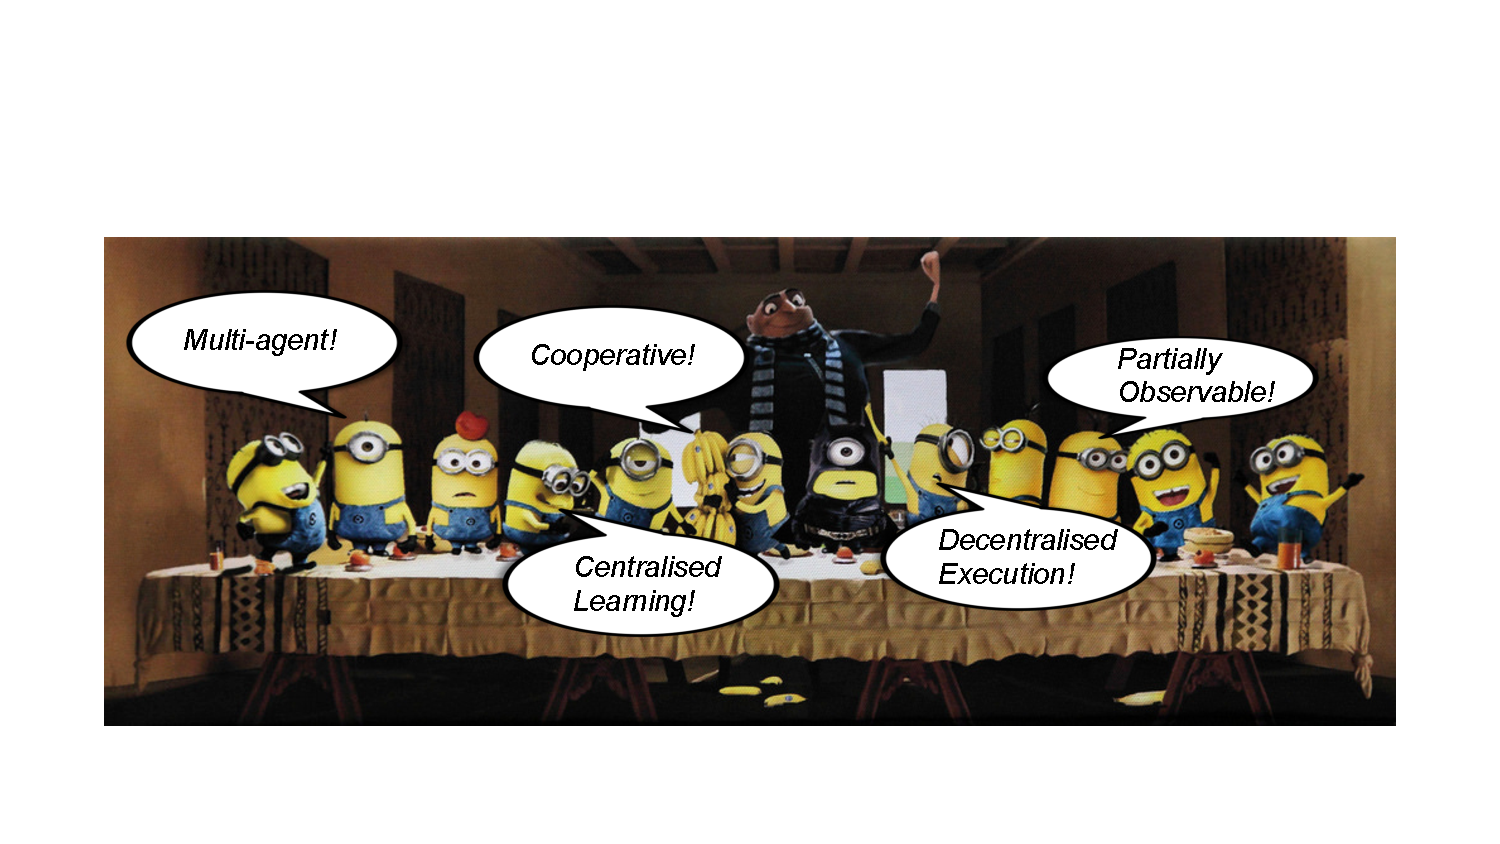
\includegraphics[scale = 0.55]{setting}\\ \ \\
  (Figure by Jakob Foerster)
\end{center} 

}

\frame{
\frametitle{Markov Decision Process}
%%%%%%%%%%%%%%%%%

\begin{itemize}
	\item Agent observes  \sw{state} $s \in S$ and selects an \sw{action} $u \in U$
	\vspace{3mm}	
	\item State transitions: $P(s'|s,u): S \times U \times S \rightarrow [0,1]$
	\vspace{3mm}	
	\item Receives \sw{reward}: $r(s,u): S \times U \rightarrow \mathbb{R}$
	\vspace{3mm}	
	\item Goal: maximise expected cumulative discounted \sw{return}:
	\begin{equation*}
		R_t = \sum_{k=0}^\infty \gamma^k r_{t+k}		
	\end{equation*}
	\item \sw{Value functions} given policy $\pi(s,u)$:
	\begin{equation*}
		V^\pi(s) = \exs{\pi}{R_t | s_t = s}~~\textup{and}~~Q^\pi(s,u) = \exs{\pi}{R_t | s_t = s, u_t=u}
	\end{equation*}
\end{itemize}
}

\frame{
\frametitle{Multi-Agent MDP}
%%%%%%%%%%%%%%%%%

\begin{itemize}
	\item All agents see the global state $s$
	\vspace{5mm}	
	\item Individual actions: $u^a \in U$
	\vspace{5mm}	
	\item State transitions: $P(s'|s,\mathbf{u}): S \times \mathbf{U} \times S \rightarrow [0,1]$
	\vspace{5mm}	
	\item Shared team reward: $r(s,\mathbf{u}): S \times \mathbf{U} \rightarrow \mathbb{R}$
	\vspace{5mm}	
	\item Equivalent to an MDP with a factored action space
\end{itemize}
}

\frame{
\frametitle{Dec-POMDP}
%%%%%%%%%%%%%%%%%

\begin{itemize}
	\item Observation function: $O(s, a): S \times A \rightarrow Z$
	\vspace{5mm}	
	\item Action-observation history: $\tau^a \in T \equiv (Z \times U)^{*}$
	\vspace{5mm}	
	\item Decentralised policies: $\pi^a(u^a|\tau^a): T \times U \rightarrow [0,1]$
	\vspace{5mm}	
	\item Natural decentralisation: communication and sensory constraints
	\vspace{5mm}	
	\item Artificial decentralisation: improve tractability
	\vspace{5mm}	
	\item Centralised learning of decentralised policies
\end{itemize}
}

\frame{
\frametitle{Setting}
%%%%%%%%%%%%%%%%%

\begin{center}
  
\includegraphics[scale = 0.55]{ct_dc}\\ \ \\
  
\includegraphics[scale = 0.35]{1} \\ \ \\
  
\includegraphics[scale = 0.35]{2} \\ \ \\  
\end{center} 

}

\frame{
\frametitle{The Predictability / Exploitation Dilemma}
%%%%%%%%%%%%%%%%%
\begin{itemize}
\item Exploitation:
\begin{itemize}
\vspace{2mm}
	\item Maximising performance requires collecting reward
\vspace{2mm}
	\item In a single-agent setting, this requires \bld{exploiting} observations
\end{itemize}
\vspace{2mm}
\item Predictability:	
\vspace{2mm}
\begin{itemize}
	\item Dec-POMDP agents cannot explicitly communicate
\vspace{2mm}
	\item Coordination requires \bld{predictability}:``stick to the plan!''
\vspace{2mm}
	\item Predictability can require ignoring private information 
\end{itemize}
\vspace{4mm}
\end{itemize}
\begin{center}
\emph{When does the benefit of exploiting private\\observations outweigh the cost in predictability?}
\end{center}
}

\frame{
\frametitle{Independent Learning}
%%%%%%%%%%%%%%%%%
\begin{itemize}
	\item Independent $Q$-learning [Tan 1993]
	\begin{itemize}
	\item Each agent learns independently with its own $Q$-function
	\item Treats other agents as part of the environment
	\end{itemize}
	\vspace{5mm}
	\item Independent actor-critic [Foerster et al.\ 2018]
	\begin{itemize}
	\item Each agent learns independently with its own actor-critic
	\item Treats other agents as part of the environment
	\end{itemize}
	\vspace{5mm}	
	\item Speed learning with \sw{parameter sharing}
	\begin{itemize}
	\item Different inputs, including $a$, induce different behaviour
	\item Still independent: value functions condition only on $\tau^a$ and $u^a$
	\end{itemize}
	\vspace{5mm}
	\item Limitations:
	\begin{itemize}
	\item Nonstationary learning
	\item Hard to learn to coordinate
	\end{itemize}
\end{itemize}
}

%\frame{
%\frametitle{Counterfactual Multi-Agent Policy Gradients (COMA) [Foerster et al.\ 2018]}
%%%%%%%%%%%%%%%%%%
%\begin{itemize}
%	\item Centralised critic: stabilise learning to coordinate
%	\vspace{7mm}
%	\item Counterfactual baseline: tackle multi-agent credit assignment
%	\vspace{7mm}
%	\item Efficient critic representation: scale to large NNs
%\end{itemize}
%}

\frame{
\frametitle{Centralised Critics {\small [Lowe et al.\ 2017; Foerster et al.\ 2018]}}
%%%%%%%%%%%%%%%%%
\vspace{2mm}
\centering Centralised $V(s,\boldsymbol{\tau})$ or $Q(s,\boldsymbol{\tau},\mathbf{u}) \rightarrow$ hard greedification $\rightarrow$ actor-critic\\
\vspace{-2mm}	
\begin{center}
  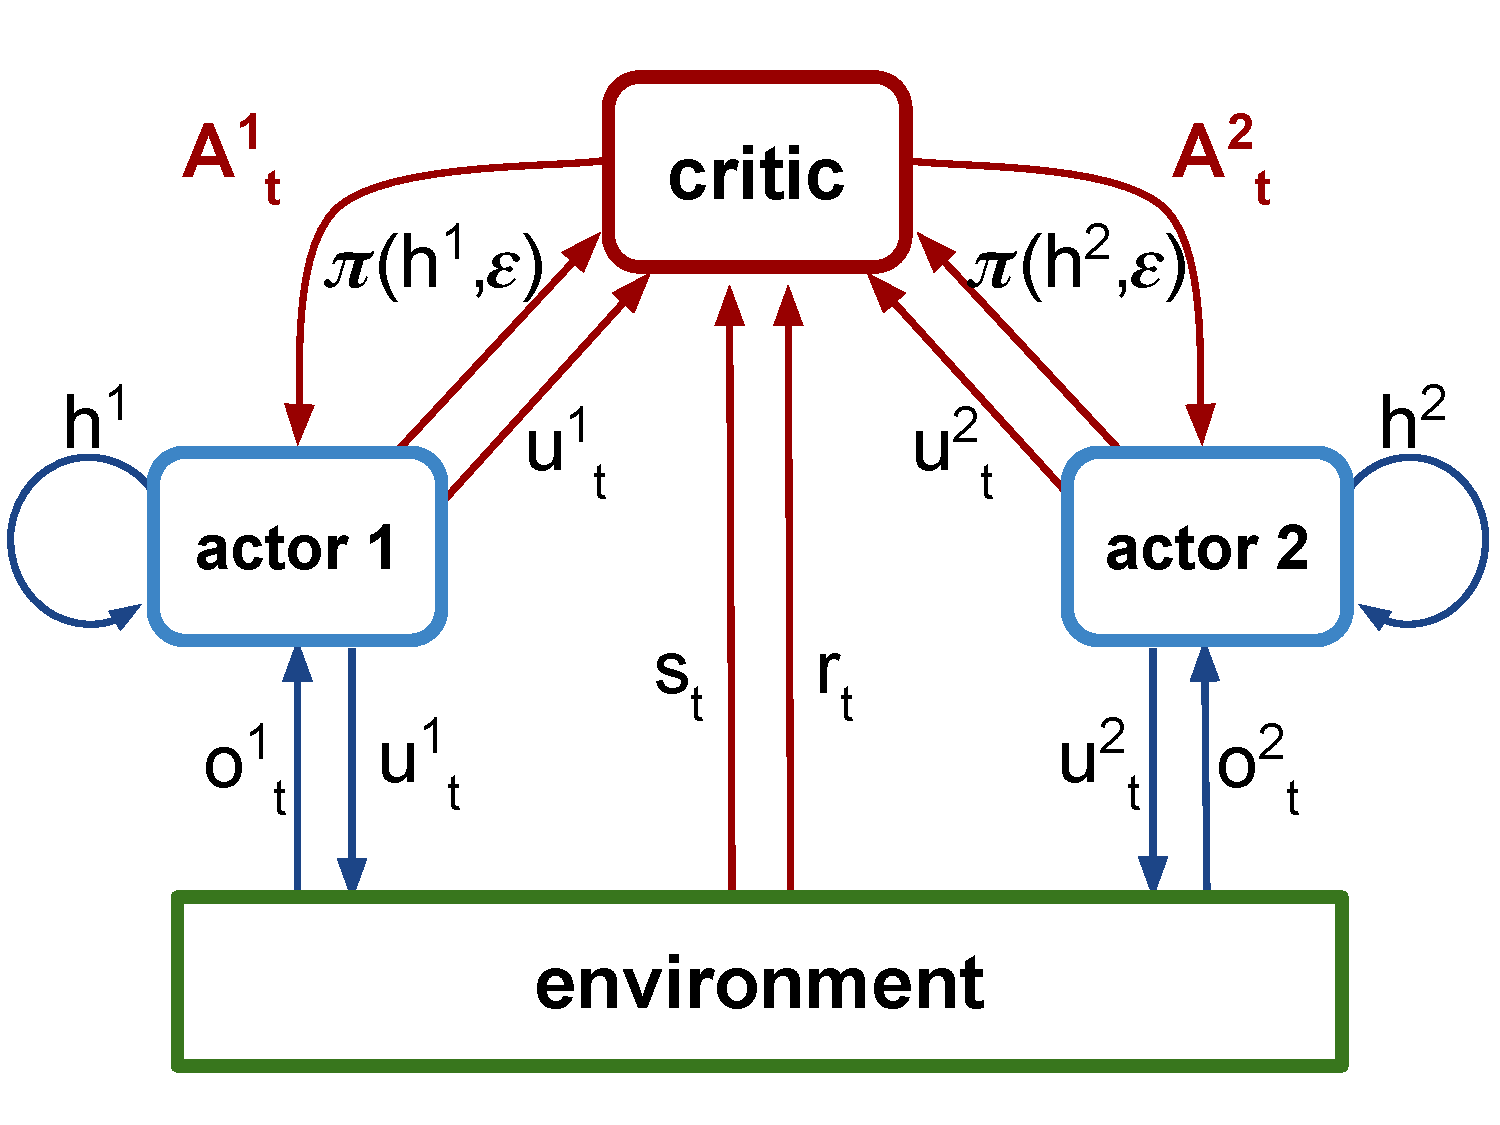
\includegraphics[scale = 0.4]{coma_architecture}
\end{center} 
}
%
%\frame{
%\frametitle{Wonderful Life Utility [Wolpert \& Tumer 2000]}
%%%%%%%%%%%%%%%%%%
%
%\begin{center}
%  
\includegraphics[scale = 0.2]{its-a-wonderful-life}
%\end{center} 
%
%}
%
%\frame{
%\frametitle{Difference Rewards [Tumer \& Agogino 2007]}
%%%%%%%%%%%%%%%%%%
%\begin{itemize}
%	\item Per-agent shaped reward:
%	\begin{equation*}
%		D^a(s,\mathbf{u}) = r(s,\mathbf{u}) - r(s, (\mathbf{u}^{-a},c^a))
%	\end{equation*}
%	where $c^a$ is a \sw{default action}
%	\vspace{5mm}
%	\item Important property:
%	\begin{equation*}
%	D^a(s,(\mathbf{u}^{-a},\dot{u}^a)) > D^a(s,\mathbf{u}) \implies r(s,(\mathbf{u}^{-a},\dot{u}^a)) > r(s, (\mathbf{u}^{-a},a))		
%	\end{equation*} 
%	\vspace{1mm}
%	\item Limitations:
%	\begin{itemize}
%	\vspace{2mm}
%	\item Need (extra) simulation to estimate counterfactual $r(s, (\mathbf{u}^{-a},c^a))$
%	\vspace{2mm}
%	\item Need expertise to choose $c^a$
%	\end{itemize}
%\end{itemize}
%}
%
%\frame{
%\frametitle{Counterfactual Baseline}
%%%%%%%%%%%%%%%%%%
%\begin{itemize}
%\item Use $Q(s,\mathbf{u})$ to estimate difference rewards:
%\begin{align*}
%	g_a(\tau) &= \sum_{t=0}^{T} \nabla_{\theta} \log \pi_\theta (u^a_t \vert \tau^a_t)A^a(s_t,\mathbf{u}_t)\\
%	A^a(s, \mathbf{u}) &= Q(s, \mathbf{u} ) - \sum_{u^a} \pi^a(u^a \vert \tau^a) Q(s,(\mathbf{u}^{-a},u^a))
%\end{align*}
%\item Baseline takes expectation wrt $u^a$
%\vspace{5mm}
%\item Critic obviates need for extra simulations
%\vspace{5mm}
%\item Expectation wrt action obviates need for default
%\end{itemize}
%
%}
%
%\frame{
%\frametitle{Efficient Critic Representation}
%%%%%%%%%%%%%%%%%%
%%\begin{itemize}
%%	\item If $Q(s, \mathbf{u})$ is a deep NN, evaluation is expensive
%%	\item Naive representation yields NN with $|U|^n$ outputs
%%\end{itemize}
%%\vspace{-3mm}
%\begin{center}
%  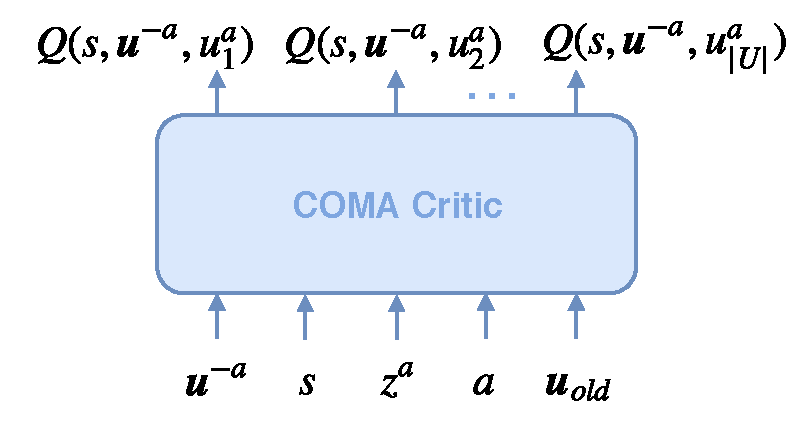
\includegraphics[scale = 0.8]{COMA-Critic.pdf}
%\end{center} 
%%\vspace{-7mm}
%%\begin{itemize}
%%	\item Need only one forward pass
%%	\item NN has only $|U|$ outputs
%%\end{itemize}
%}
%
%\frame{
%\frametitle{Starcraft}
%%%%%%%%%%%%%%%%%%
%\begin{center}
%  
\includegraphics[scale = 0.4]{starcraft-original}
%\end{center} 
%}
%
%\frame{
%\frametitle{Starcraft Micromanagement [Synnaeve et al.\ 2016]}
%%%%%%%%%%%%%%%%%%
%\begin{center}
%  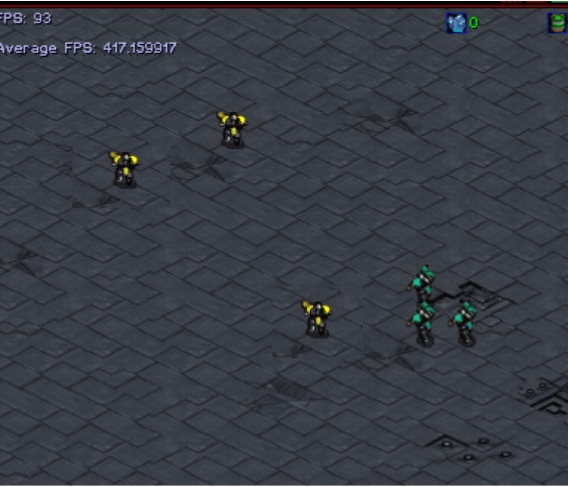
\includegraphics[scale = 0.4]{ps_old}
%\end{center} 
%}
%
%
%\frame{
%\frametitle{Decentralised Starcraft Micromanagement}
%%%%%%%%%%%%%%%%%%
%
%\begin{center}
%  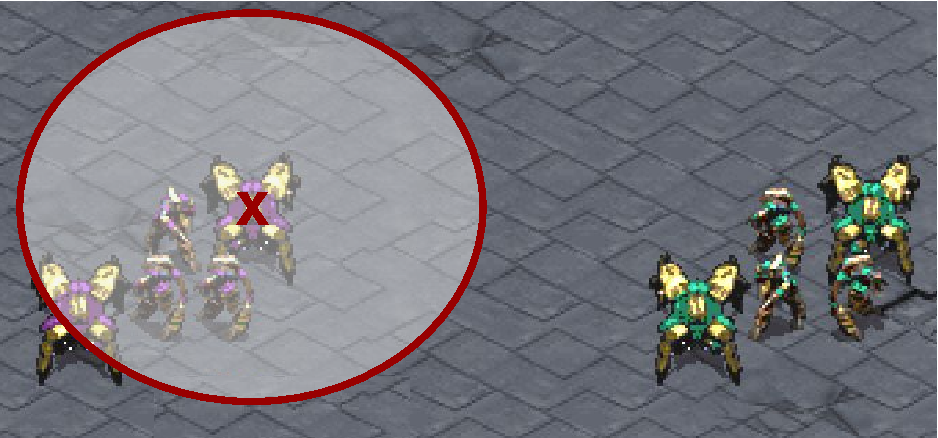
\includegraphics[scale = 0.5]{unites_start}
%\end{center} 
%
%}
%
%\frame{
%\frametitle{Baseline Algorithms}
%%%%%%%%%%%%%%%%%%
%\begin{itemize}
%	\item \sw{IAC-V:} independent actor-critic with $V(\tau^a)$ (TD error)
%	\vspace{5mm}
%	\item \sw{IAC-Q:} independent actor-critic with $A(\tau^a, u^a) = Q(\tau^a,u^a)  - V(\tau^a)$
%	\vspace{5mm}
%	\item \sw{Central-V:} centralised critic $V(s)$ (TD error)
%	\vspace{5mm}
%	\item \sw{Central-QV:} 
%	\begin{itemize}
%	\vspace{2mm}
%	\item Centralised critics $Q(s,\mathbf{u})$ and $V(s)$
%	\vspace{2mm}
%	\item Advantage gradient $A(s, \mathbf{u}) = Q(s, \mathbf{u}) - V(s)$
%	\vspace{2mm}
%	\item COMA but with $b(s) = V(s)$
%	\end{itemize}
%\end{itemize}
%}
%
%\frame{
%\frametitle{COMA Results vs.\ Baselines (Average Performance)}
%%%%%%%%%%%%%%%%%%
%\begin{figure}
%	\centering
%	\vspace{-3mm}
%	\subfigure[3 Marines]{
%		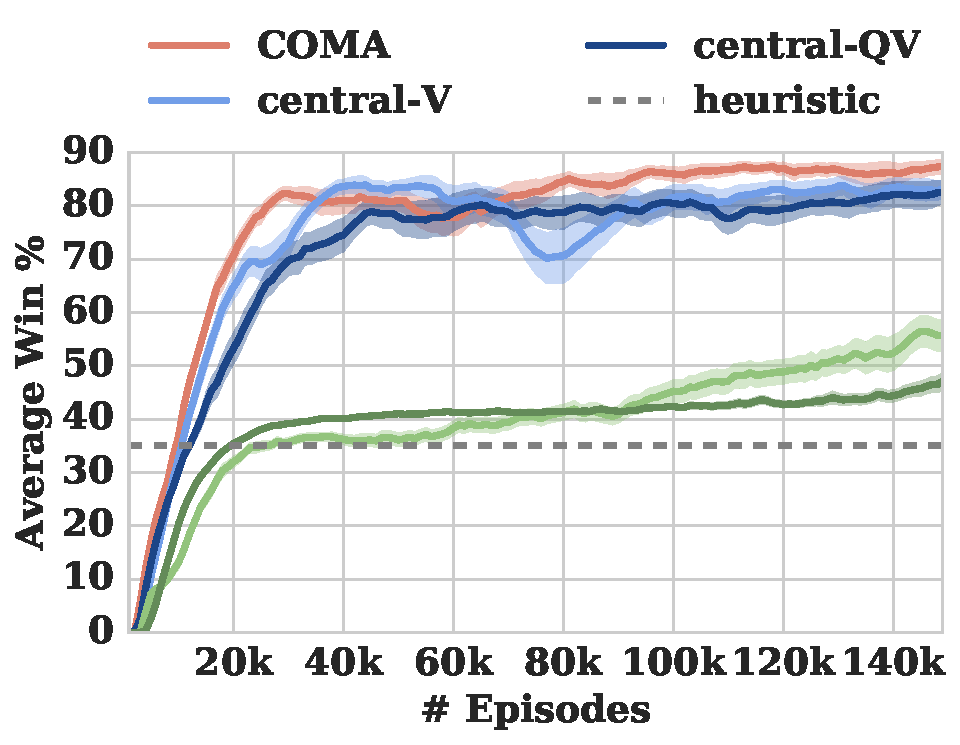
\includegraphics[width=0.4\columnwidth]{test_per_win_avg_mean_m3v3_4plots}
%	}
%	\subfigure[5 Marines]{
%		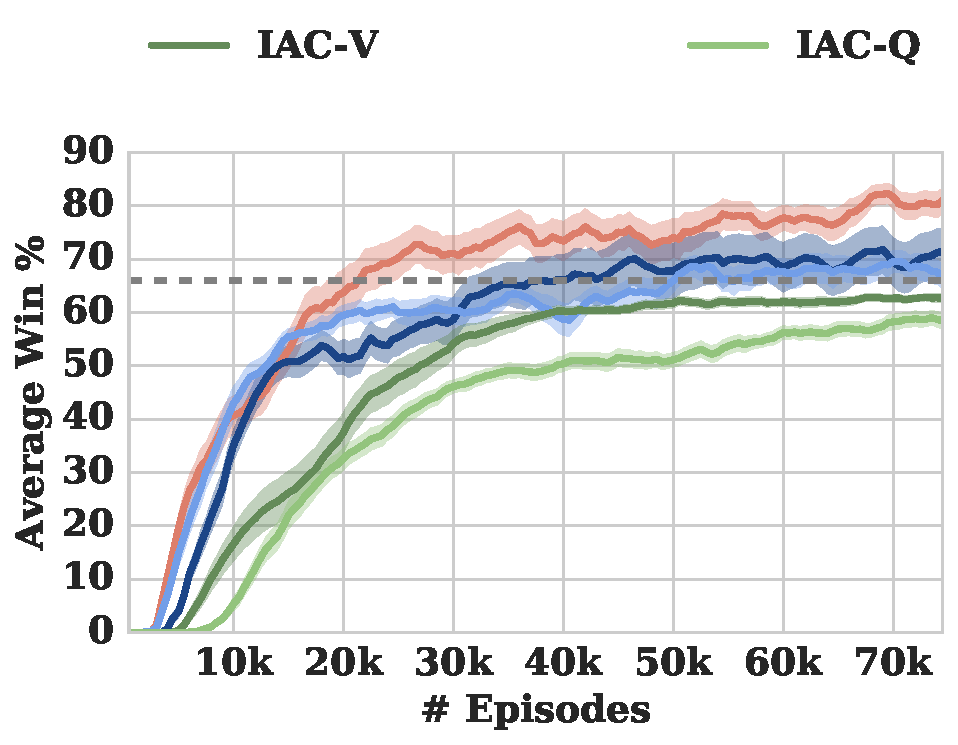
\includegraphics[width=0.4\columnwidth]{test_per_win_avg_mean_m5v5_4plots}
%	}
%%	\vspace{-4mm}
%	\subfigure[5 Wraiths]{
%		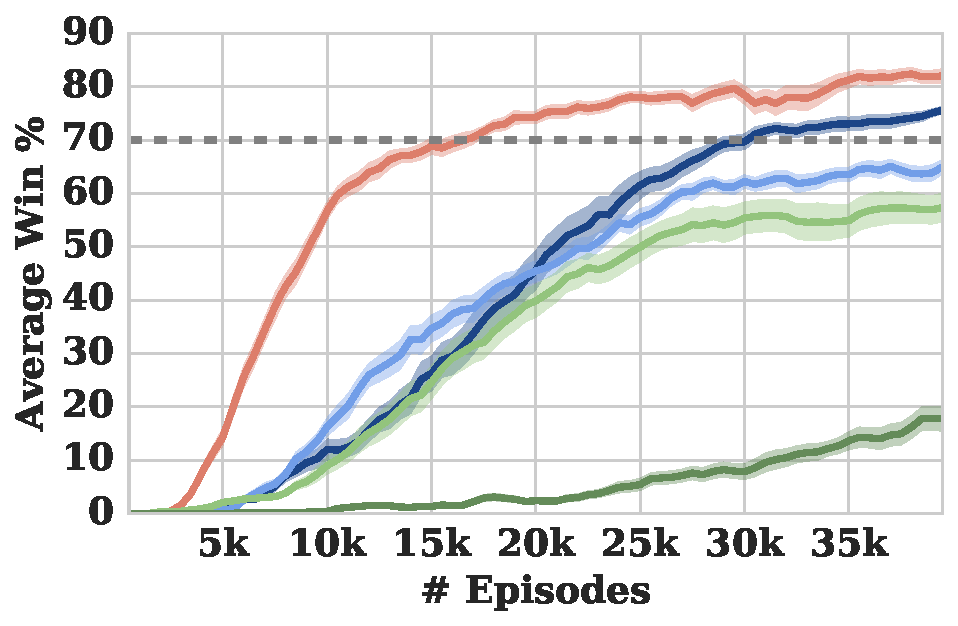
\includegraphics[width=0.4\columnwidth]{test_per_win_avg_mean_w5v5_4plots} 
%	}
%	\subfigure[2 Dragoons \& 3 Zealots]{
%		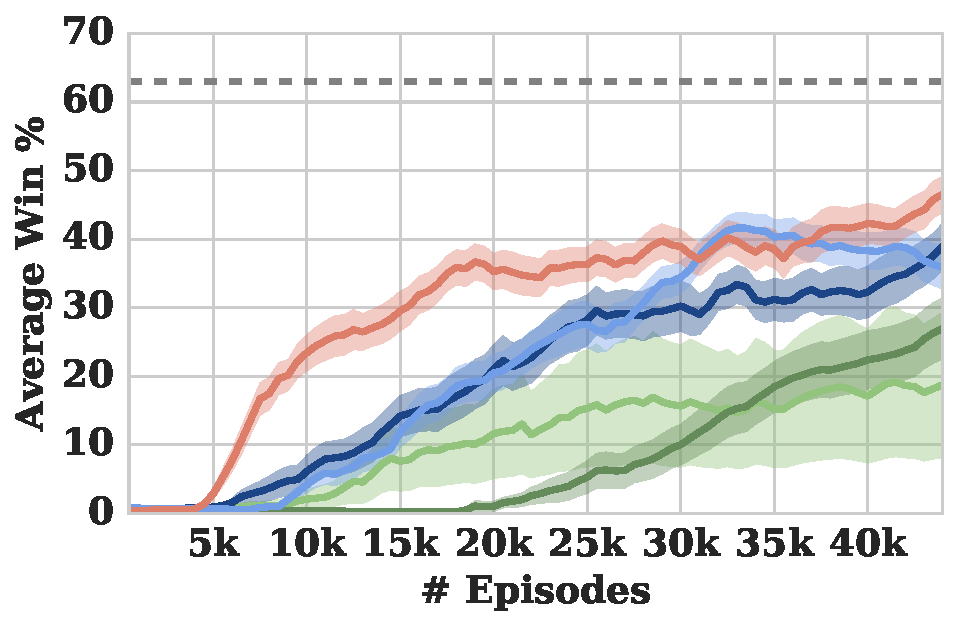
\includegraphics[width=0.4\columnwidth]{test_per_win_avg_mean_dragoons_zealots_4plots} 
%	}
%\end{figure}
%}
%
%\frame{
%\frametitle{COMA Results vs.\ Centralised (Best Agents)}
%%%%%%%%%%%%%%%%%%
%
%	\begin{center}
%		\resizebox{\textwidth}{!}{
%			\begin{tabular}{ccccc}
%				\toprule
%				\multirow{2}{*}{Map}  &
%				\multirow{2}{*}{COMA}  & \multirow{2}{*}{Heuristic} & 
%				\multirow{2}{*}{DQN} & \multirow{2}{*}{GMEZO}  \\ \ \\
%								
%				\midrule
%				3 Marines         &  98  &  74  &   - & -          \\
%				5 Marines       &  95  &  98  &  99 & 100 \\
%				5 Wraiths*       &  98  &  82  &    70 & 
%				74 \\
%				2 Dragoons \& 3 Zealots      &  65  &  68  &    61 & 90 \\
%				\bottomrule
%				
%			\end{tabular}
%		}
%				
%	\end{center}
%}
%
%\frame{
%\frametitle{Paper}
%%%%%%%%%%%%%%%%%%
%
%\center
%{\bf Counterfactual Multi-Agent Policy Gradients} \\ \ \\
%
%Jakob Foerster, Gregory Farquhar, Triantafyllos Afouras, \\ Nantas Nardelli, and Shimon Whiteson \\ \ \\
%
%{\bf The Outstanding Student Paper of AAAI-18}
%
%}

\frame{
\frametitle{Factored Joint Value Functions}
%%%%%%%%%%%%%%%%%
\begin{itemize}
	\item \sw{Factored value functions} [Guestrin et al.\ 2003] can improve scalability:
		\begin{equation*}
Q_{tot}(\boldsymbol{\tau}, \mathbf{u}; \boldsymbol{\theta}) = \sum_{e=1}^E Q_e (\mathbf{\tau}^e, \mathbf{u}^e;\mathbf{\theta}^e)
	\end{equation*}
	where each $e$ indicates a subset of the agents
\end{itemize}
\begin{center}
  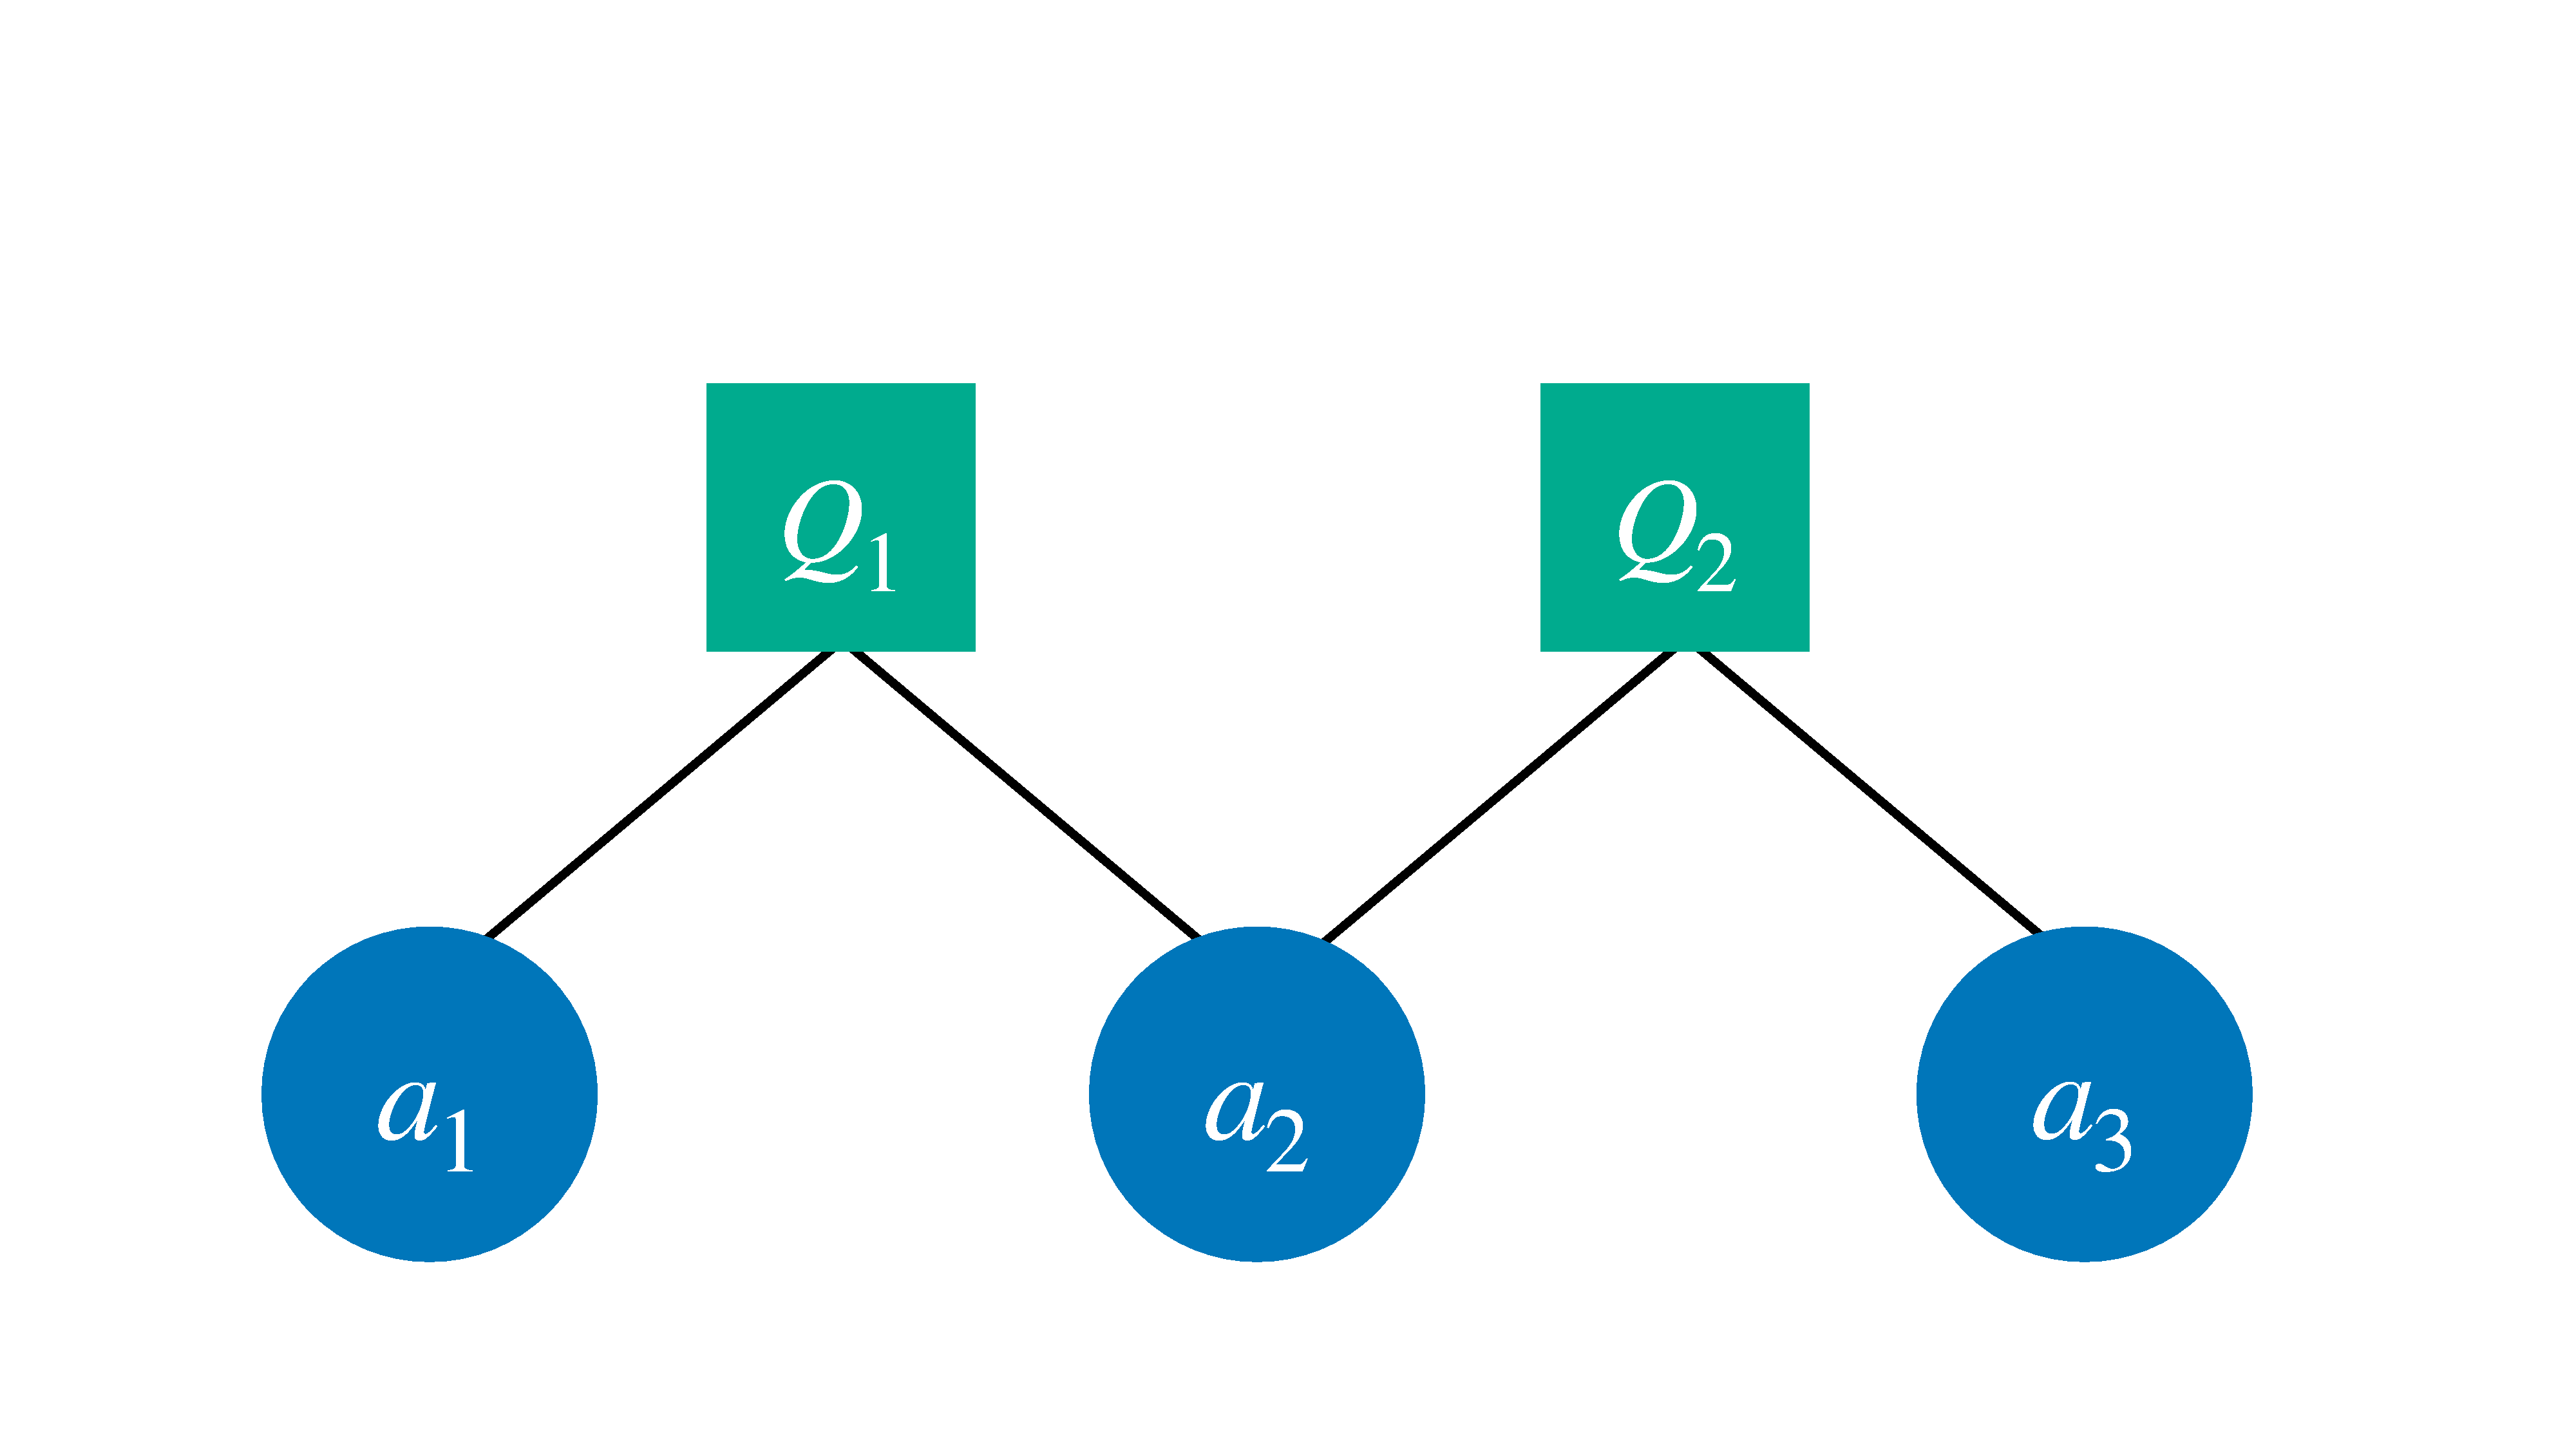
\includegraphics[scale = 0.15]{factor-graph.pdf}\\ \ \\
\end{center} 
}

\frame{
\frametitle{Value Decomposition Networks {\small [Sunehag et al., 2017]}}
%%%%%%%%%%%%%%%%%
\begin{itemize}
	\item Most extreme factorisation: one per agent:
	\begin{equation*}
Q_{tot}(\boldsymbol{\tau}, \mathbf{u}; \boldsymbol{\theta}) = \sum_{a=1}^N Q_a (\tau^a, u^a;\theta^a)
	\end{equation*}
	\vspace{0.2cm}
\end{itemize}
\begin{center}
  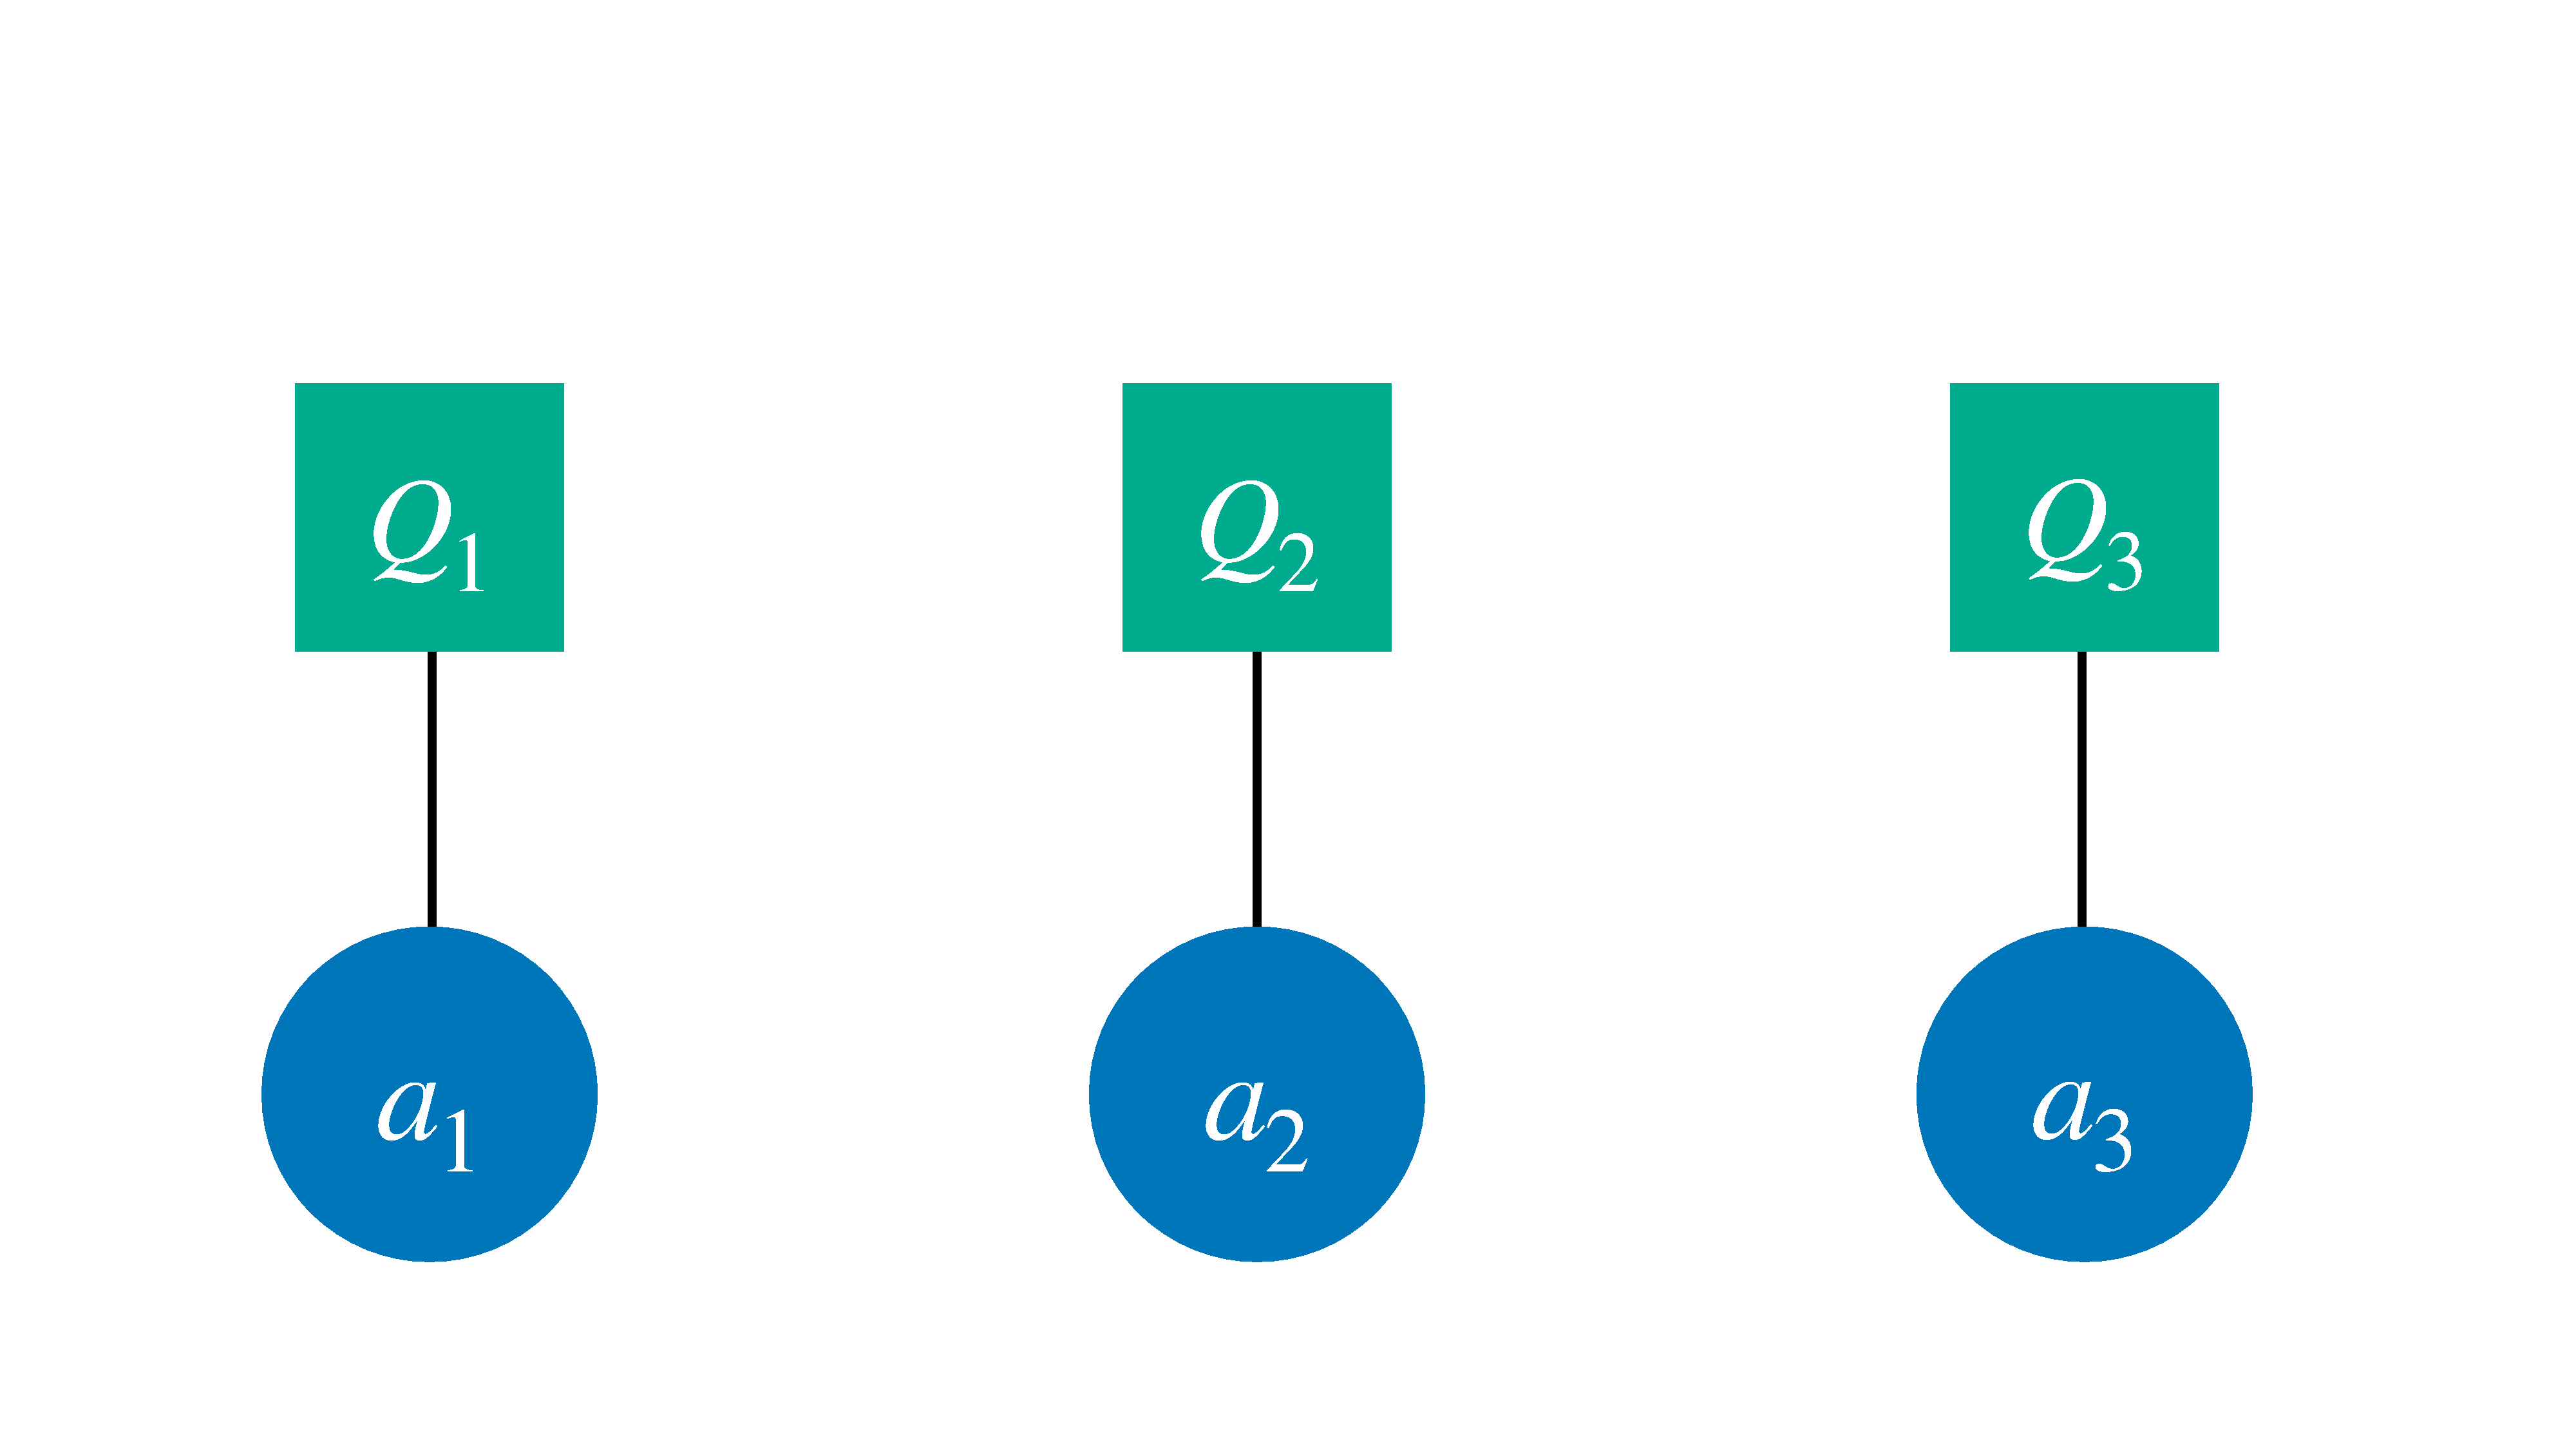
\includegraphics[scale = 0.15]{VDN.pdf}\\ \ \\
\end{center} 
}
	
	
\frame{
\frametitle{Decentralisability}
%%%%%%%%%%%%%%%%%
\begin{itemize}
	\item Added benefit of decentralising the $\max$ and $\argmax$:
	\begin{align*}
	\max_{\mathbf{u}}Q_{tot}(\boldsymbol{\tau}, \mathbf{u}; \boldsymbol{\theta}) &= \sum \max_{u^a}Q_a(\tau^a, u^a; \theta^a) \\ \ \\
	\argmax_{\mathbf{u}}Q_{tot}(\boldsymbol{\tau}, \mathbf{u}; \boldsymbol{\theta}) &= 
	\begin{pmatrix}
	\argmax_{u^1}Q_1(\tau^1, u^1; \theta^1)   \\
	\vdots \\
	\argmax_{u^n}Q_n(\tau^n, u^n; \theta^n) \\
	\end{pmatrix}
	\end{align*}
	\vspace{2mm}
	\item No more hard greedification $\implies Q$-learning, not actor-critic:
	\begin{align*}
\mathcal{L}(\boldsymbol{\theta})&=\sum\limits_{i=1}^{b}\left[\left(y_i^{\text{tot}}-Q_{tot}(\boldsymbol{\tau}, \mathbf{u}; \boldsymbol{\theta})\right)^2\right],\\
y^{\text{tot}}_i&=r_i+\gamma\max_{\mathbf{u}^\prime}Q_{tot}(\boldsymbol{\tau}^\prime_i, \mathbf{u}^\prime; \boldsymbol{\theta^-})
\end{align*} 
\end{itemize}
}

\frame{
\frametitle{QMIX's Monotonicity Constraint}
%%%%%%%%%%%%%%%%%
\vspace{2mm}
	To decentralise $\max/\argmax$, it suffices to enforce:
$
	\frac{\partial Q_{tot}}{\partial Q_a}  \geq 0,~ \forall a \in A
$

\begin{center}
  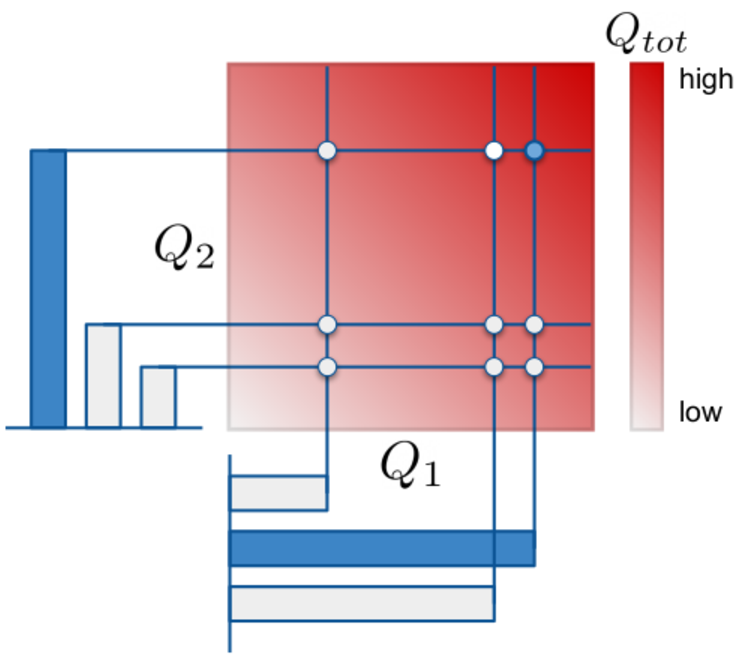
\includegraphics[scale = 0.6]{monotonic_2}
\end{center} 	

}

\frame{
\frametitle{Representational Capacity}
%%%%%%%%%%%%%%%%%

\begin{center}
	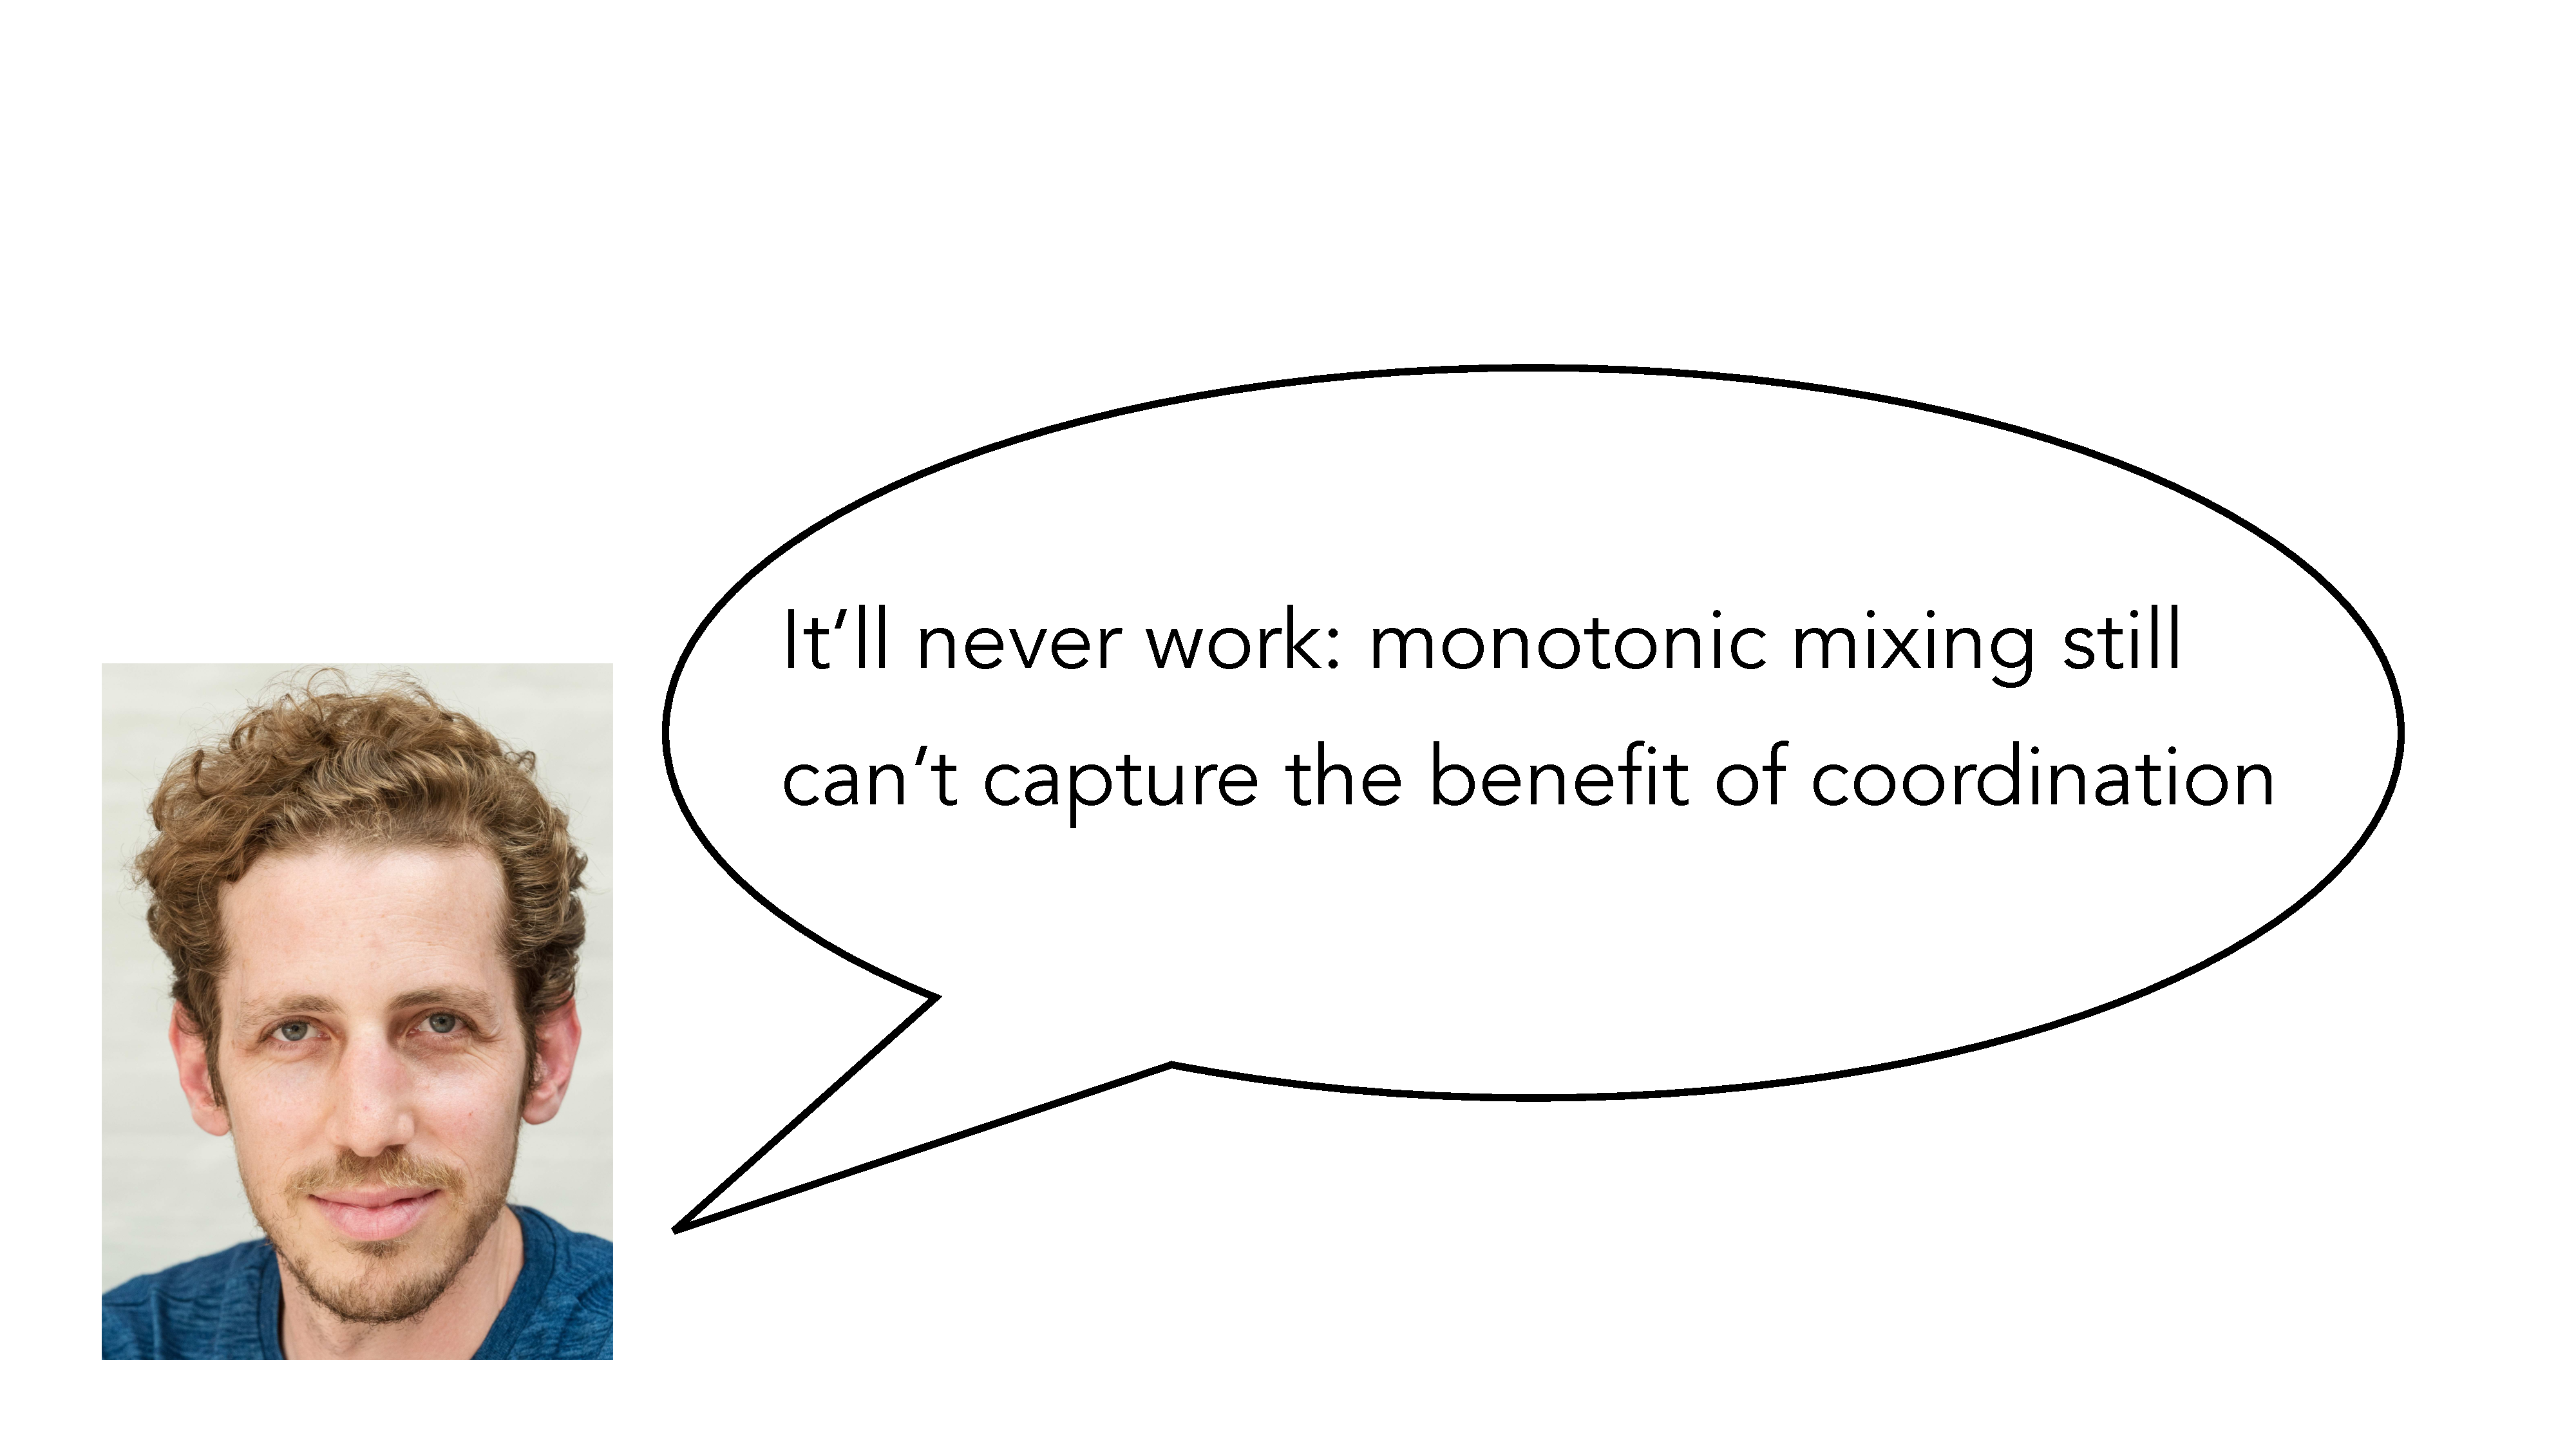
\includegraphics[width=0.7\textwidth]{Shimon}\\
	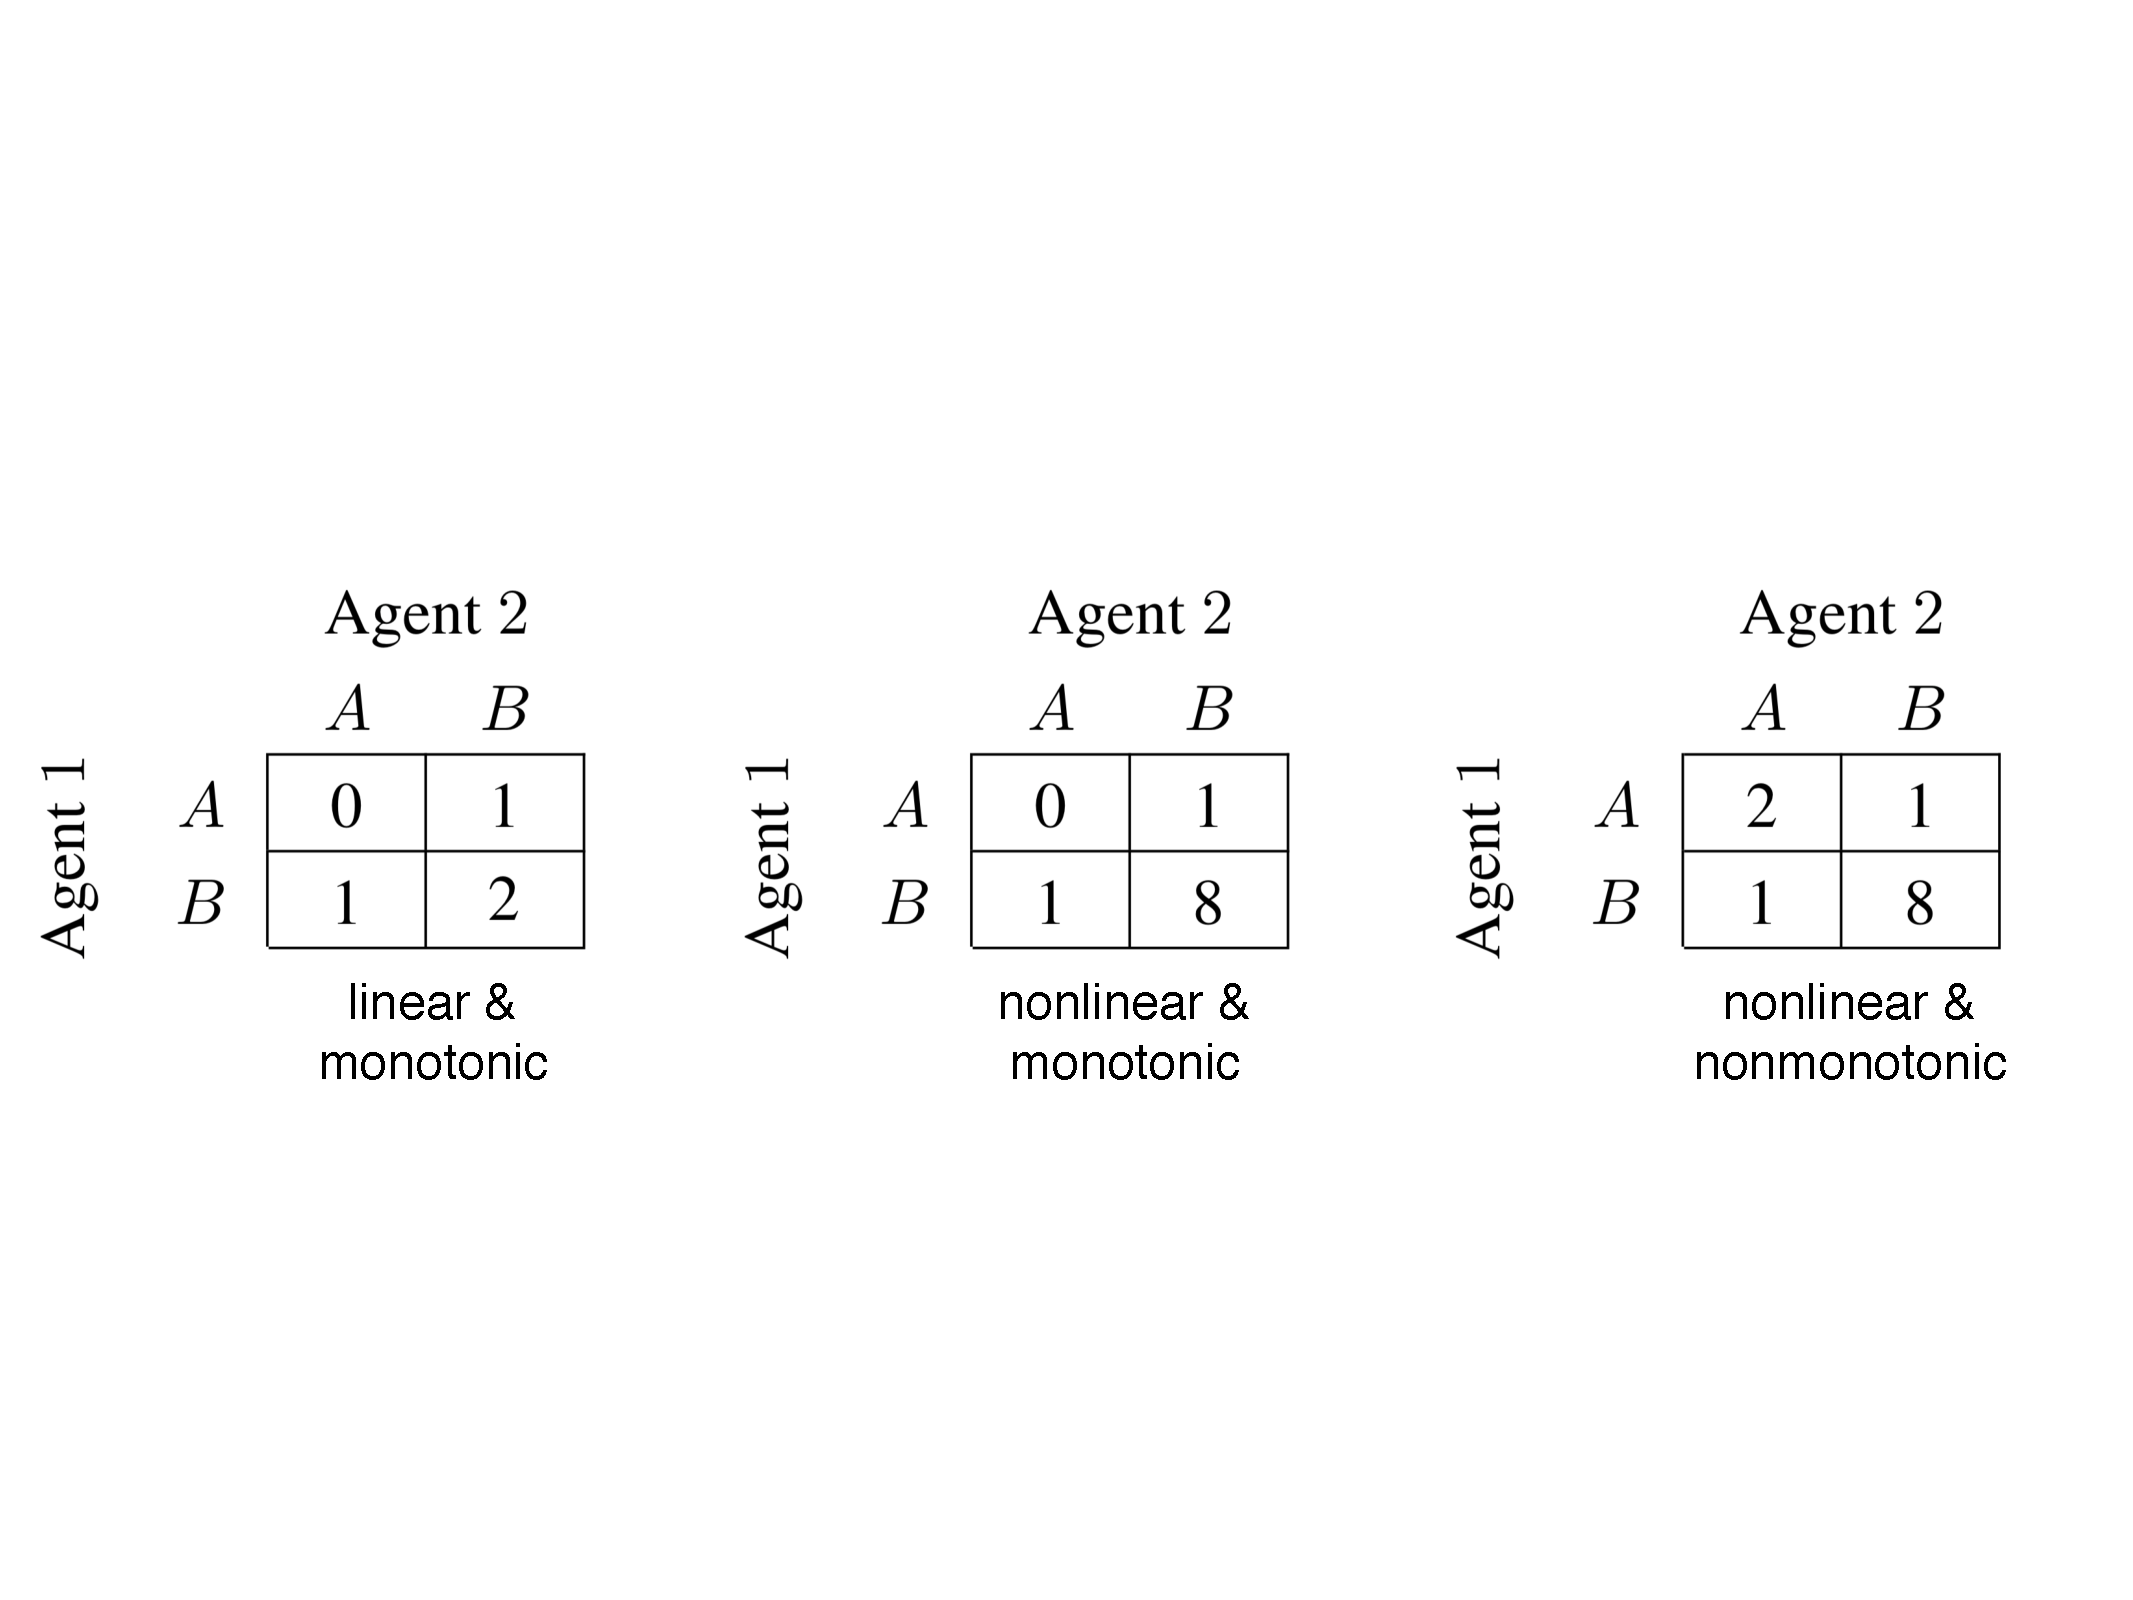
\includegraphics[width=\textwidth]{games.pdf}
\end{center}
\ \ \ \ \ \ \ \ \ VDN \& QMIX \ \ \ \ \ \ \ \ \ \ \ \ \ \ \ \ \ Just QMIX \ \ \ \ \ \ \ \ \ \ \ \ \ \ \ \ \ \ \ \ \ \ Neither\\ \ \\
}

\frame{
\frametitle{Bootstrapping}
%%%%%%%%%%%%%%%%%
\begin{center}
	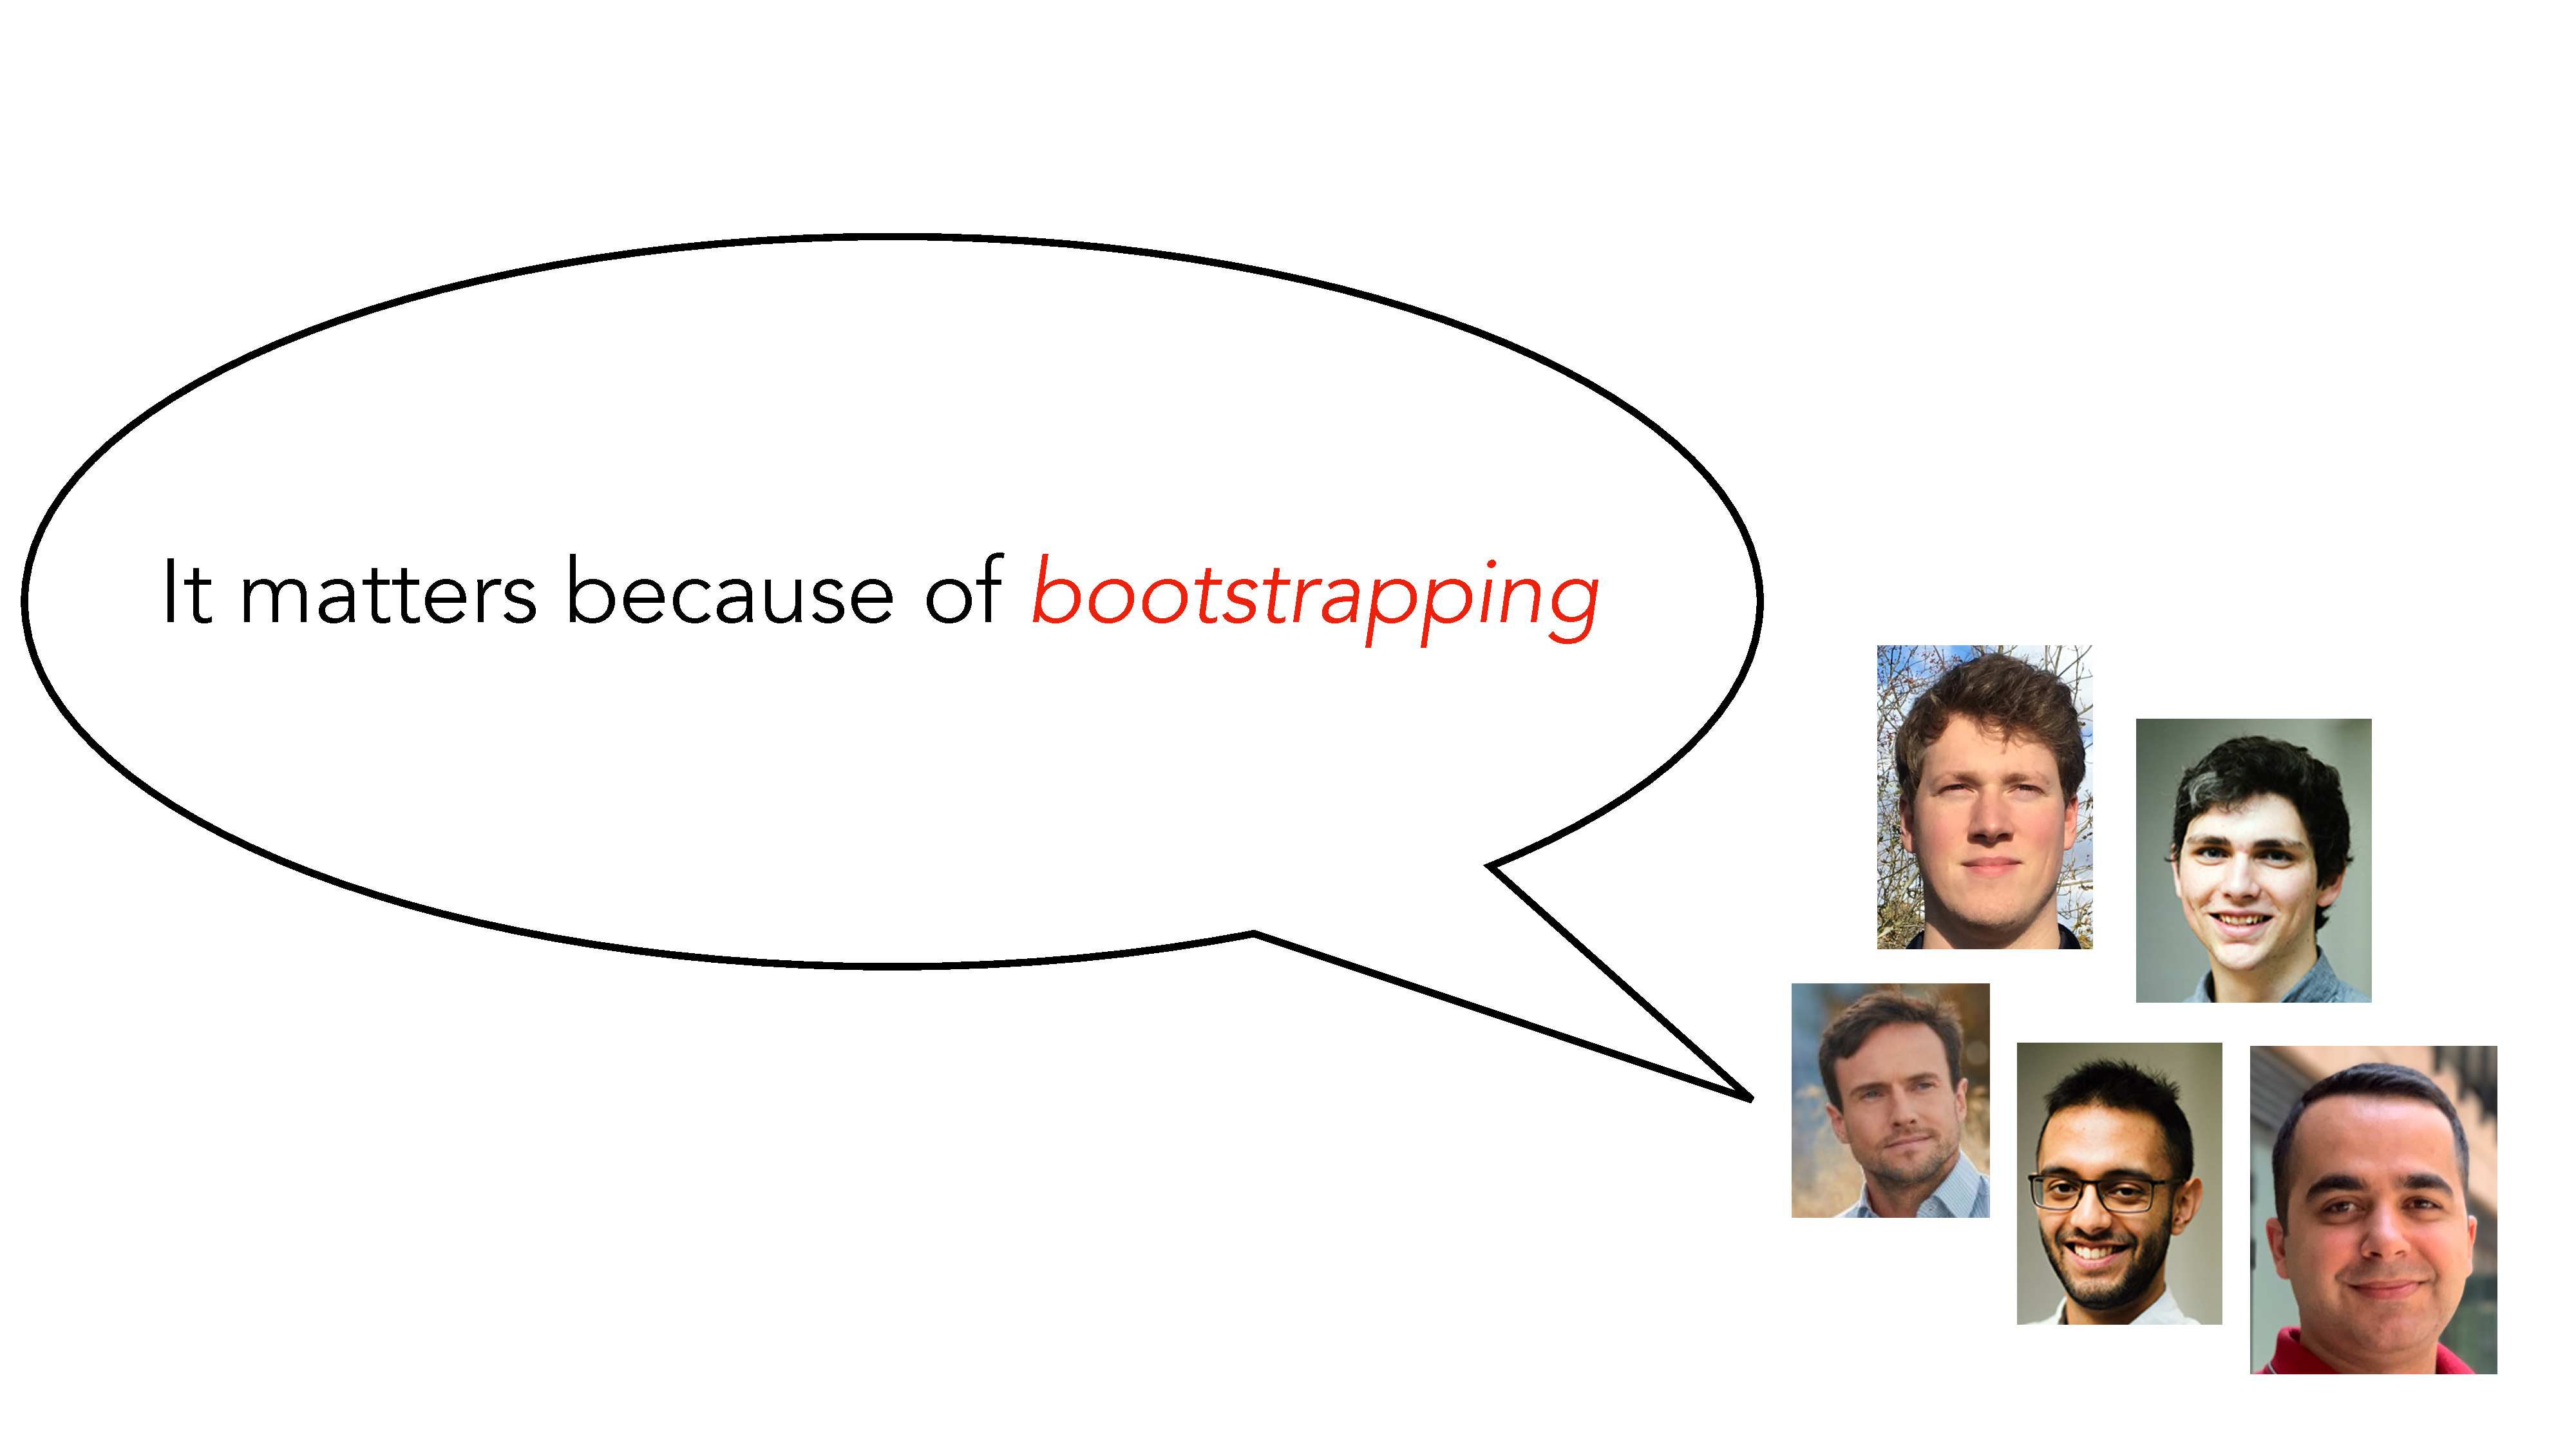
\includegraphics[width=\textwidth]{Students}\\
\end{center}
\vspace{-2mm}
		\begin{align*}
\mathcal{L}(\boldsymbol{\theta})&=\sum\limits_{i=1}^{b}\left[\left(y_i^{\text{tot}}-Q_{tot}(\boldsymbol{\tau}, \mathbf{u}, s; \boldsymbol{\theta})\right)^2\right],\\
y^{\text{tot}}_i&=r_i+\gamma\max_{\mathbf{u}^\prime}\textcolor{red}{Q_{tot}(\boldsymbol{\tau}^\prime_i, \mathbf{u}^\prime, s^\prime; \boldsymbol{\theta^-})}
\end{align*} 
}

\frame{
\frametitle{Two-Step Game}
%%%%%%%%%%%%%%%%%
\vspace{-2mm}
\begin{center}	
	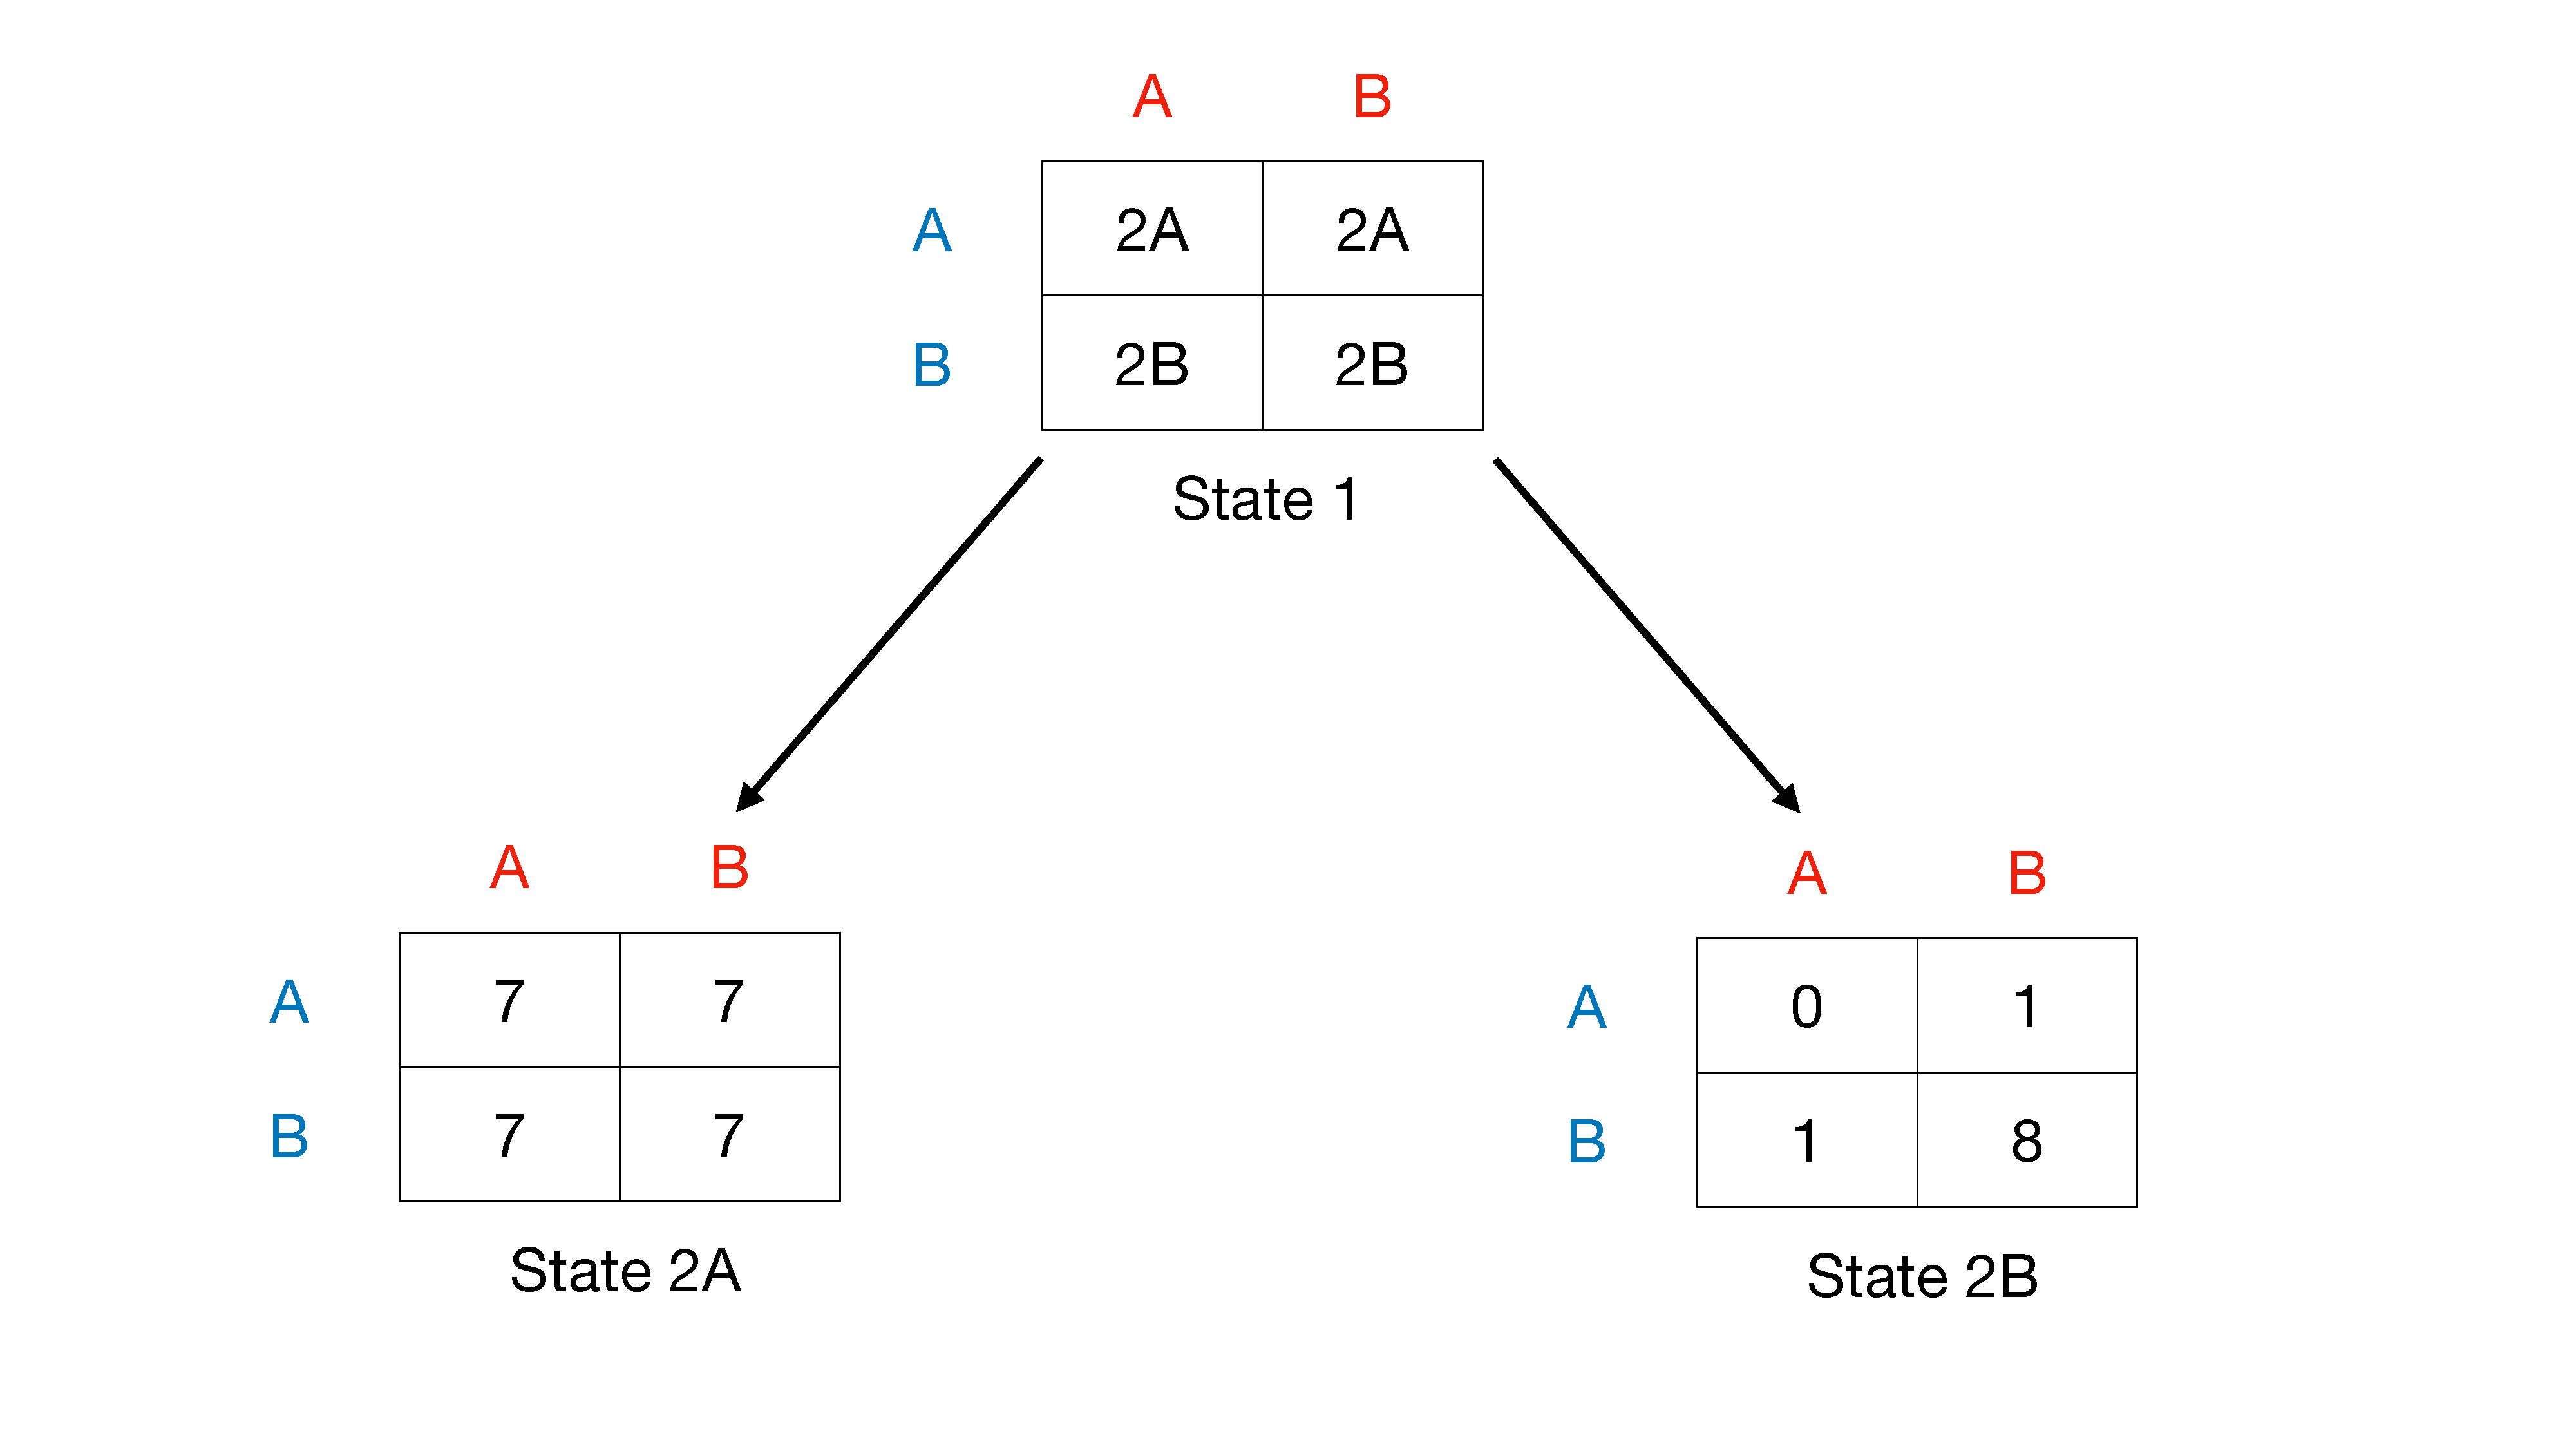
\includegraphics[width=\textwidth]{2step.pdf} 
\end{center}
}

\frame{
\frametitle{Two-Step Game Results}
%%%%%%%%%%%%%%%%%
\vspace{-2mm}
\begin{center}	
	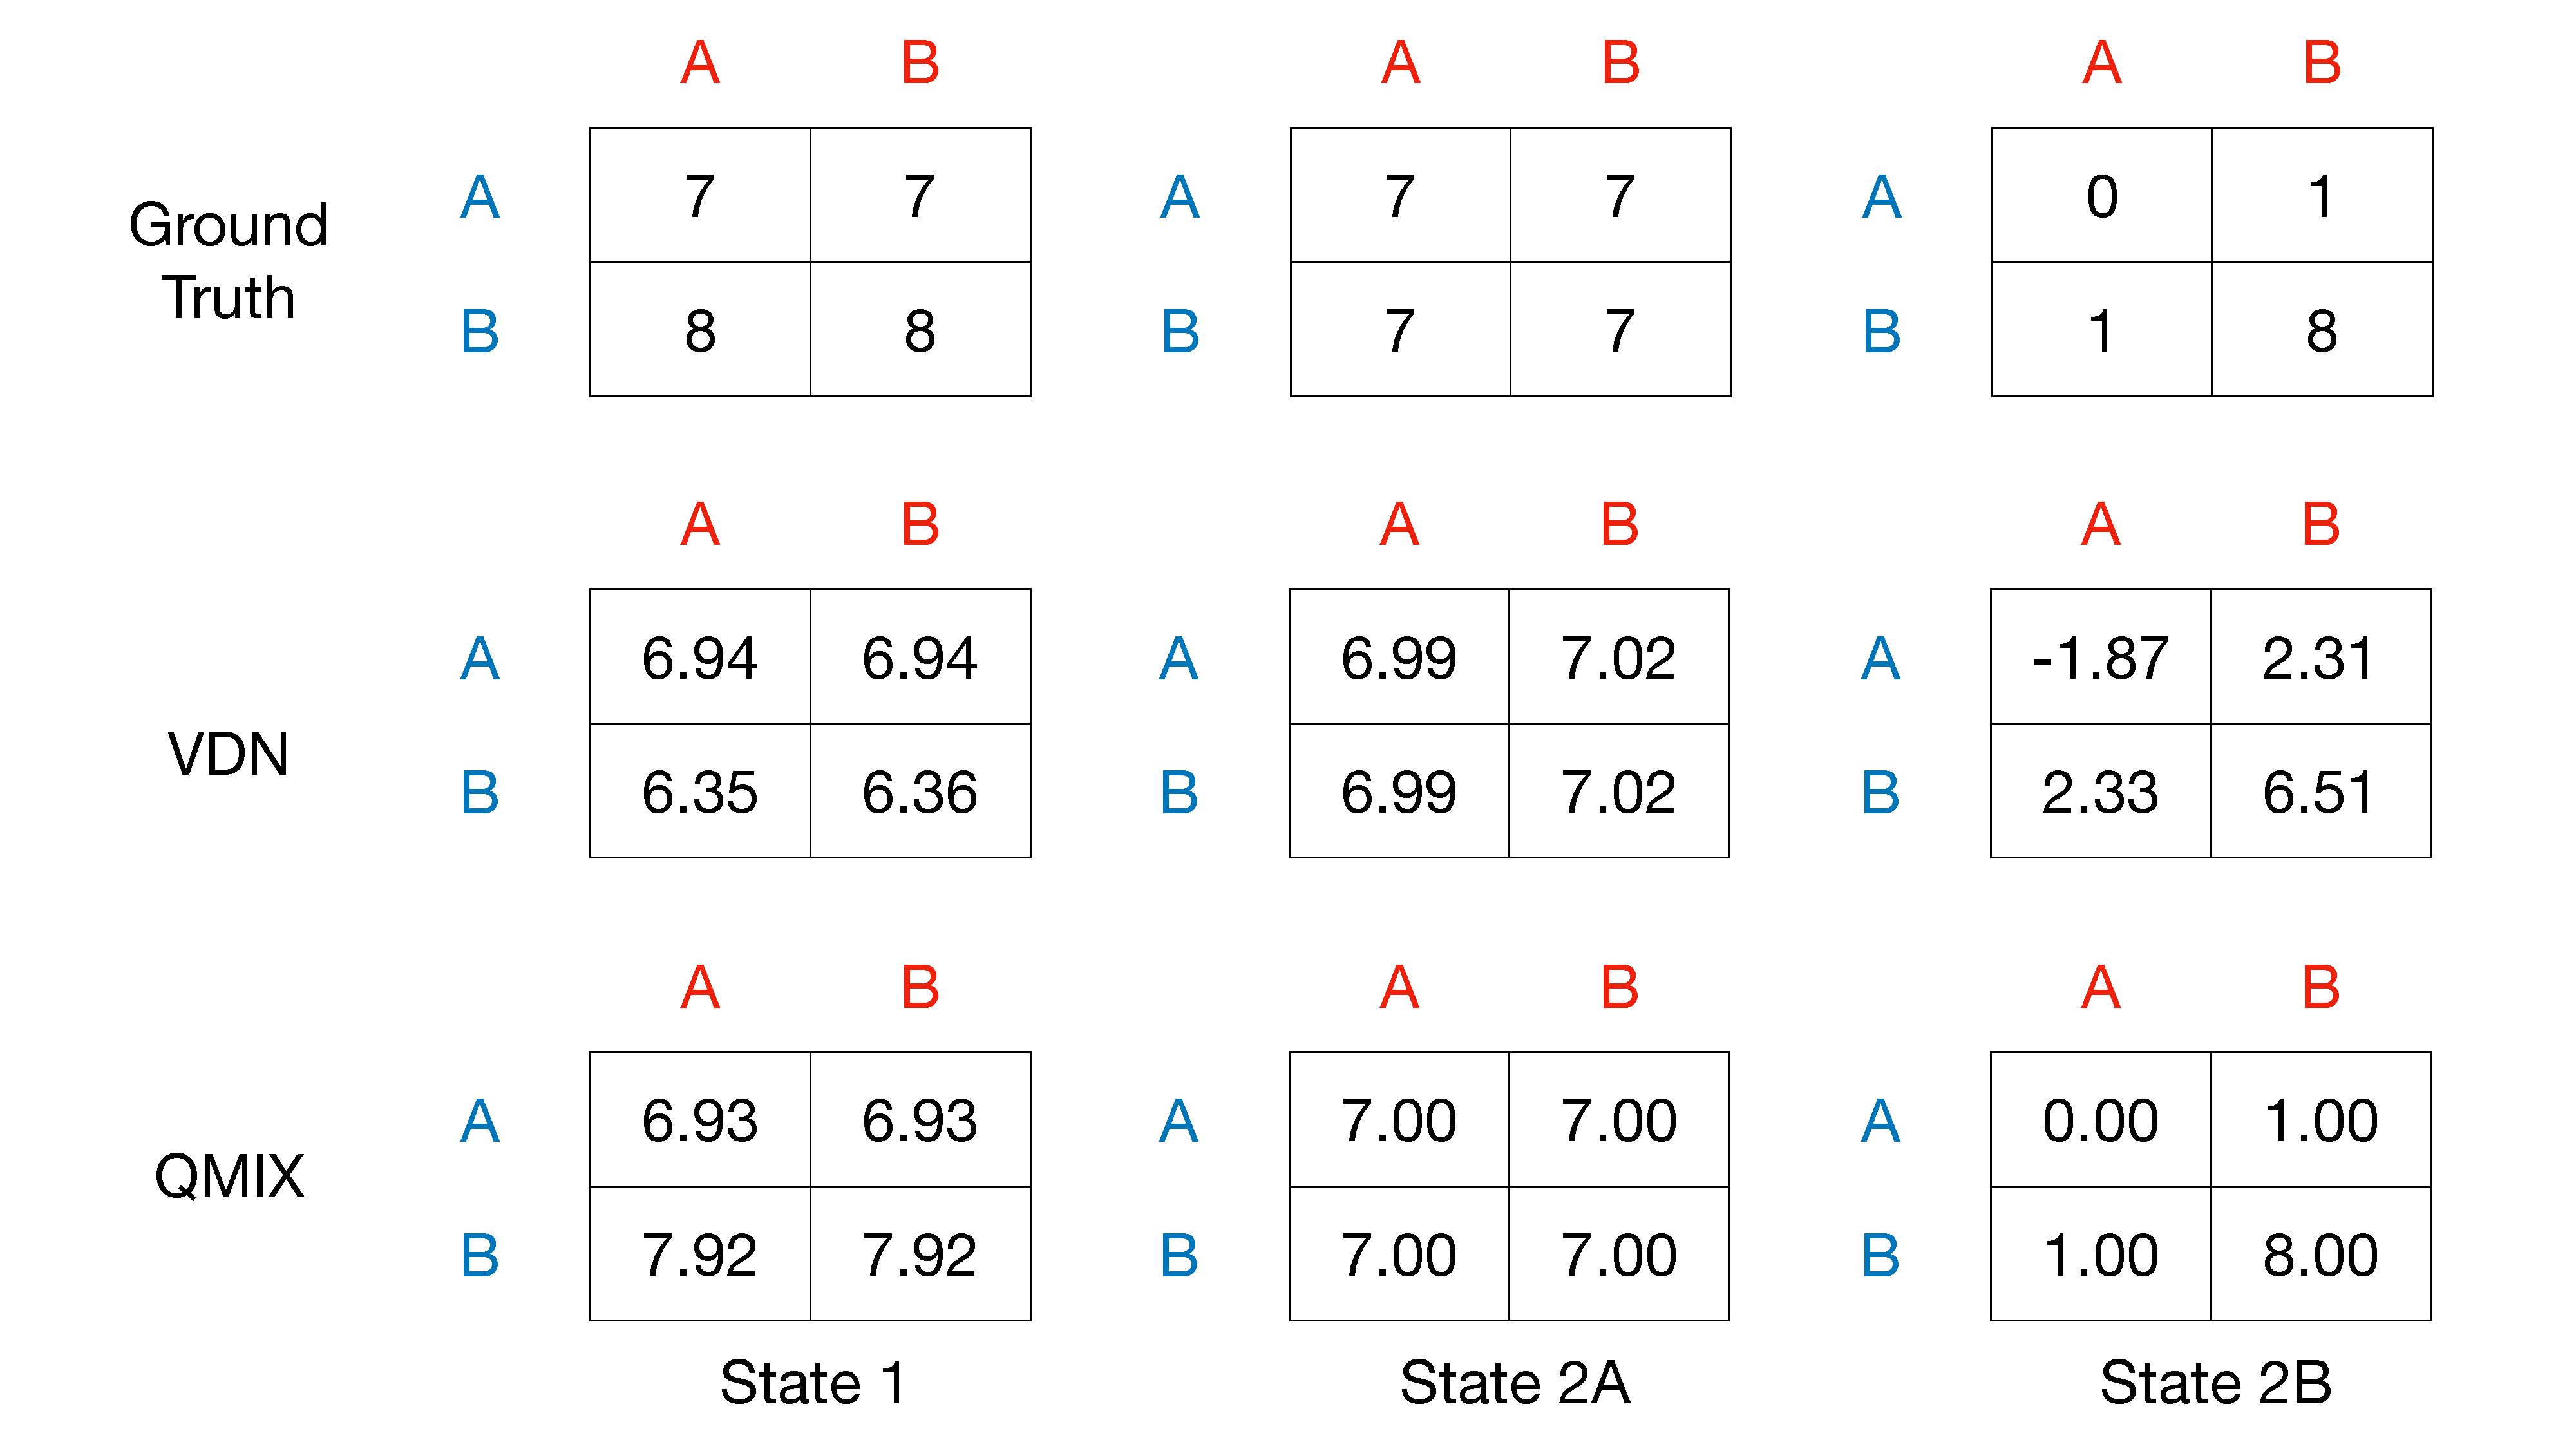
\includegraphics[width=\textwidth]{2step-results.pdf} 
\end{center}
}

\frame{
\frametitle{QMIX [Rashid et al.\ 2018]}
%%%%%%%%%%%%%%%%%
\vspace{-0.2cm}
\begin{center}
  \includegraphics[width=\textwidth]{All_Three_Blow_up.png}
\end{center} 	
	\begin{itemize}
		\item Agent network: represents $Q_i (\tau^a, u^a;\theta^a)$
		\vspace{2mm}
		\item Mixing network: represents $Q_{tot}(\boldsymbol{\tau})$ using nonnegative weights
		\vspace{2mm}		
		\item Hypernetwork: generates weights of hypernetwork based on global $s$
	\end{itemize}
}

\frame{
\frametitle{Random Matrix Games (The Students Were Right)}
%%%%%%%%%%%%%%%%%
	\includegraphics[width=0.32\textwidth]{"figures/results/matrix_games/no_legend/2 Agents 2 Actions_max_qtot_median"}
	\includegraphics[width=0.32\textwidth]{"figures/results/matrix_games/no_legend/2 Agents 3 Actions_max_qtot_median"}
	\includegraphics[width=0.32\textwidth]{"figures/results/matrix_games/no_legend/2 Agents 4 Actions_max_qtot_median"}
	\includegraphics[width=0.32\textwidth]{"figures/results/matrix_games/no_legend/3 Agents 2 Actions_max_qtot_median"}
	\includegraphics[width=0.32\textwidth]{"figures/results/matrix_games/no_legend/3 Agents 3 Actions_max_qtot_median"}
	\includegraphics[width=0.32\textwidth]{"figures/results/matrix_games/no_legend/3 Agents 4 Actions_max_qtot_median"}
	\includegraphics[width=0.32\textwidth]{"figures/results/matrix_games/no_legend/4 Agents 2 Actions_max_qtot_median"}
	\includegraphics[width=0.32\textwidth]{"figures/results/matrix_games/no_legend/4 Agents 3 Actions_max_qtot_median"}
	\includegraphics[width=0.32\textwidth]{"figures/results/matrix_games/legend/4 Agents 4 Actions_max_qtot_median"}
}

\frame{
\frametitle{StarCraft Multi-Agent Challenge (SMAC)\\{\small [Samvelyan et al.\ 2019]}}
%%%%%%%%%%%%%%%%%
\begin{figure}
    \centering
        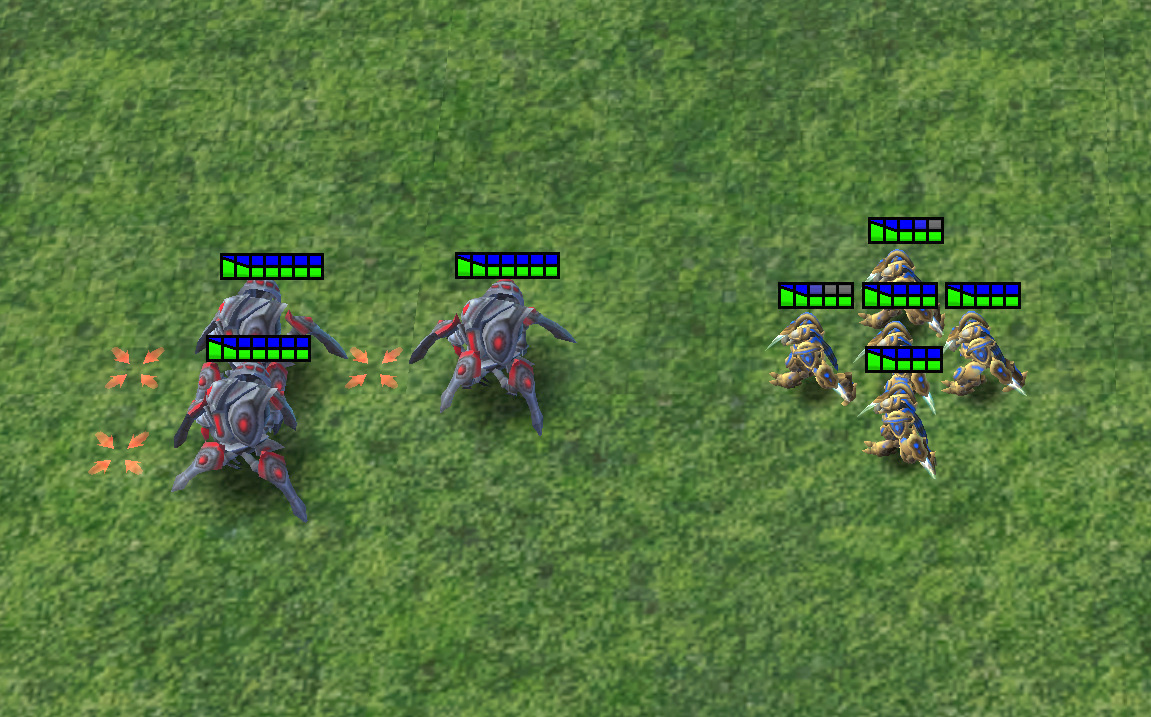
\includegraphics[width=0.32\textwidth]{3s_vs_5z.jpg}
        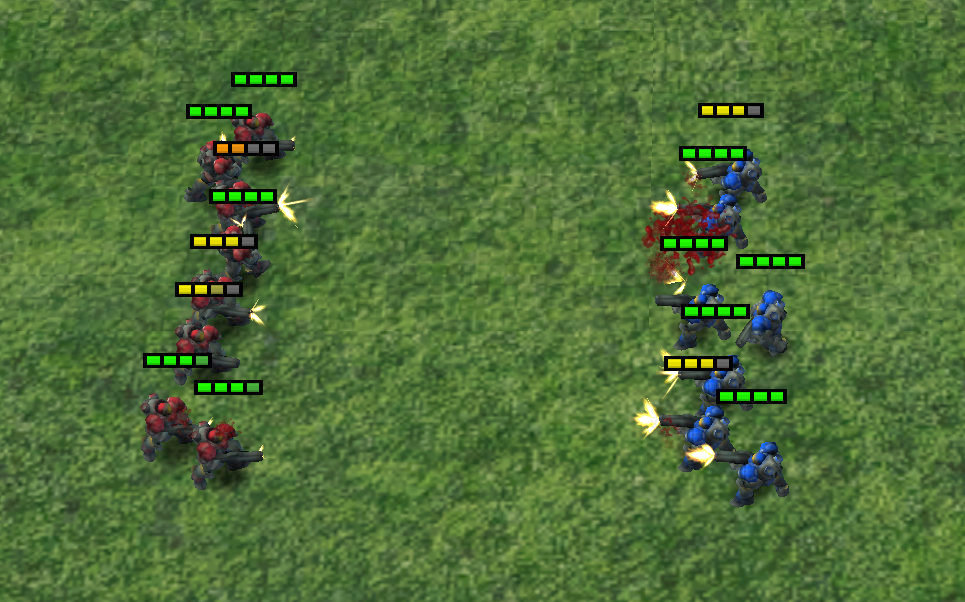
\includegraphics[width=0.32\textwidth]{8m_8m.jpg}        
        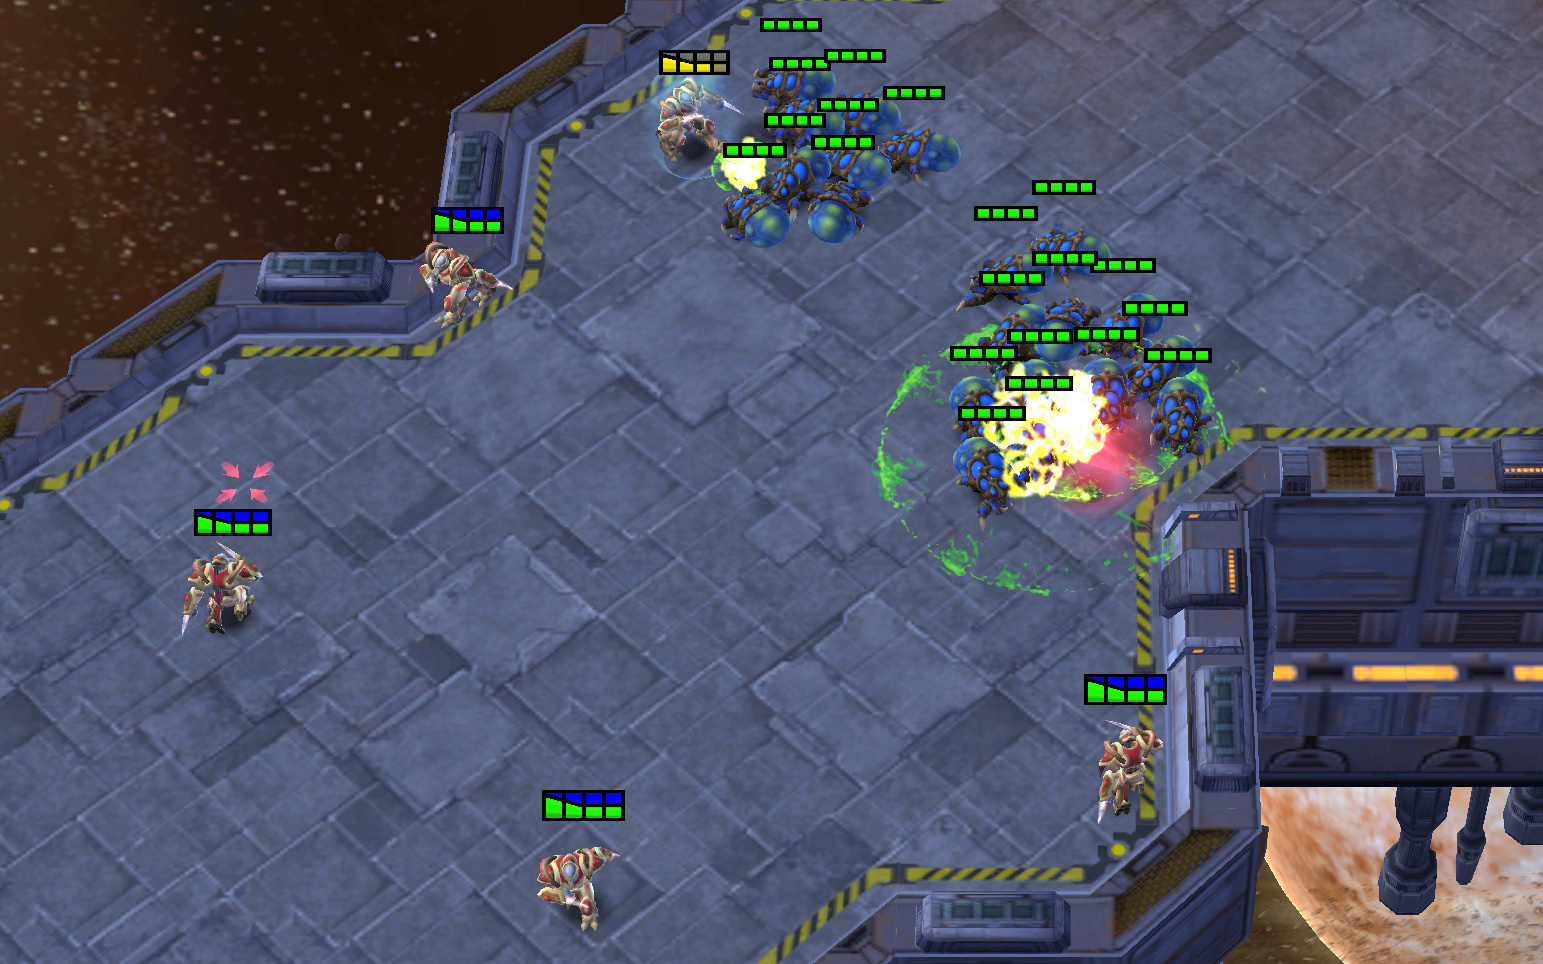
\includegraphics[width=0.32\textwidth]{banelings4.jpg}\\ \ \\               
        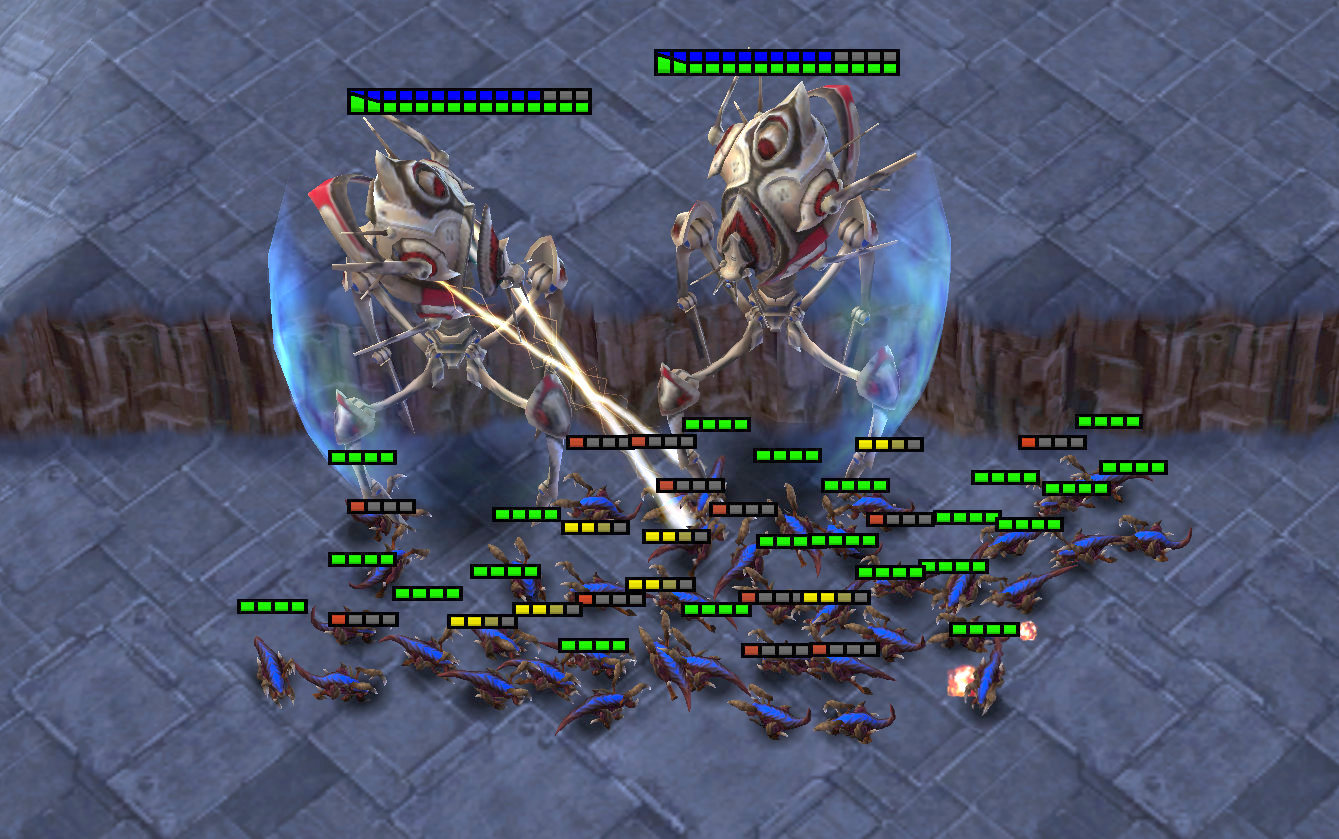
\includegraphics[width=0.32\textwidth]{micro_colossus2.jpg}                
        \includegraphics[width=0.32\textwidth]{micro_corridor.jpg}                        
        \includegraphics[width=0.32\textwidth]{MMM.jpg}
\end{figure}
\begin{center}
\url{https://github.com/oxwhirl/smac}
\url{https://github.com/oxwhirl/pymarl}	
\end{center}

}

\frame{
\frametitle{Partial Observability in SMAC}
%%%%%%%%%%%%%%%%%
\begin{center}
	\includegraphics[width=0.75\textwidth]{smac_agent_obs} \\
\vspace{0.2cm}
Cyan = sight range \ \ \ \ \ Red = shooting range
\end{center}
}

\frame{
\frametitle{SMAC Maps}
	\scalebox{.75}{
		\begin{tabular}{ccc}
			\toprule
			Name & Ally Units & Enemy Units \\
			\midrule
			\texttt{2s3z} &  2 Stalkers \& 3 Zealots &  2 Stalkers \& 3 Zealots \\
			\texttt{3s5z} &  3 Stalkers \&  5 Zealots &  3 Stalkers \&  5 Zealots \\
			\texttt{1c3s5z} &  1 Colossus, 3 Stalkers \&  5 Zealots &  1 Colossus, 3 Stalkers \&  5 Zealots \\
			\hline
			\texttt{5m\_vs\_6m} & 5 Marines & 6 Marines \\
			\texttt{10m\_vs\_11m} & 10 Marines & 11 Marines \\
			\texttt{27m\_vs\_30m} & 27 Marines & 30 Marines \\
			\texttt{3s5z\_vs\_3s6z} & 3 Stalkers \& 5 Zealots & 3 Stalkers \& 6 Zealots \\
			\texttt{MMM2} &  1 Medivac, 2 Marauders \& 7 Marines
			&  1 Medivac, 3 Marauders \& 8 Marines  \\
			\hline
			\texttt{2s\_vs\_1sc}& 2 Stalkers  & 1 Spine Crawler \\
			\texttt{3s\_vs\_5z} & 3 Stalkers & 5 Zealots \\
			\texttt{6h\_vs\_8z} & 6 Hydralisks  & 8 Zealots \\
			\texttt{bane\_vs\_bane} & 20 Zerglings \& 4 Banelings  & 20 Zerglings \& 4 Banelings \\		
			\texttt{2c\_vs\_64zg}& 2 Colossi  & 64 Zerglings \\		
			\texttt{corridor} & 6 Zealots  & 24 Zerglings \\
			\bottomrule
	\end{tabular}}
}

\frame{
\frametitle{Overall Results (The Students Were Right)}
%%%%%%%%%%%%%%%%%
\begin{center}
%	\includegraphics[width=0.475\textwidth]{figures/results/median_test_win.png}
	\includegraphics[width=\textwidth]{figures/results/maps_best.png}
\end{center}
%\ \ \ \ \ Median test win \% \ \ \ \ \ \ \ \ \ \ \ \ \ \ \ Total scenarios with best test win \%
}

\frame{
\frametitle{State Ablations}
%%%%%%%%%%%%%%%%%

\begin{figure}[h!]
    \centering
    \includegraphics[width=0.475\textwidth]{figures/results/ablations/1/3s5z_test_battle_won_mean_median.png}
    \includegraphics[width=0.475\textwidth]{figures/results/ablations/1/2c_vs_64zg_test_battle_won_mean_median.png}
    \includegraphics[width=0.475\textwidth]{figures/results/ablations/1/legend/MMM2_test_battle_won_mean_median.png}
\end{figure}
}


\frame{
\frametitle{Linear Ablations}
%%%%%%%%%%%%%%%%%

\begin{figure}[h!]
    \centering
    \includegraphics[width=0.475\textwidth]{figures/results/ablations/3/3s5z_test_battle_won_mean_median.png}
    \includegraphics[width=0.475\textwidth]{figures/results/ablations/3/2c_vs_64zg_test_battle_won_mean_median.png}
    \includegraphics[width=0.475\textwidth]{figures/results/ablations/3/legend/MMM2_test_battle_won_mean_median.png}
\end{figure}
}

\frame{
\frametitle{Learned Mixing Functions (2c\_vs\_64zg)}
%%%%%%%%%%%%%%%%%

\begin{figure}[h!]
    \centering
    \includegraphics[width=0.475\textwidth]{figures/vis/2c_64zg/2c_64zg_elu_0t.png}
    \includegraphics[width=0.475\textwidth]{figures/vis/2c_64zg/2c_64zg_elu_50t.png}
\end{figure}
\ \ \ \ \ \ \ \ \ \ \ \ \ \ \ \ \ \ \ $t=0$ \ \ \ \ \ \ \ \ \ \  \ \ \ \ \ \ \ \ \ \ \ \ \ \ \ \ \ \ \ \ \ \ \ \ \ \ \ $t=50$

}

\frame{
\frametitle{Multi-Layer Linear Mixing (Regression)}
%%%%%%%%%%%%%%%%%

\begin{figure}[h!]
    \centering
    \includegraphics[width=\textwidth]{figures/results/regression/mixing_net_parametrisation_loss.png}
\end{figure}
}

\frame{
\frametitle{Multi-Layer Linear Mixing (SMAC)}
%%%%%%%%%%%%%%%%%

\begin{figure}[h!]
    \centering
   \includegraphics[width=0.475\textwidth]{figures/results/ablations/2/2c_vs_64zg_test_battle_won_mean_median.png}
    \includegraphics[width=0.475\textwidth]{figures/results/ablations/2/legend/MMM2_test_battle_won_mean_median.png}
\end{figure}
}

\frame{
\frametitle{Tanh Activation}
%%%%%%%%%%%%%%%%%

\begin{figure}[h!]
    \centering
     \includegraphics[width=0.475\textwidth]{figures/vis/2c_64zg/2c_64zg_tanh_0t.png}
    \includegraphics[width=0.475\textwidth]{figures/vis/2c_64zg/2c_64zg_tanh_50t.png}
\end{figure}
\vspace{-4mm}
\ \ \ \ \ \ \ \ \ \ \ \ \ \ \ \ \ \ \ $t=0$ \ \ \ \ \ \ \ \ \ \  \ \ \ \ \ \ \ \ \ \ \ \ \ \ \ \ \ \ \ \ \ \ \ \ \ \ \ $t=50$
\begin{figure}
    \includegraphics[width=0.4\textwidth]{figures/results/tanh/3s5z_test_battle_won_mean_median.png}
    \includegraphics[width=0.4\textwidth]{figures/results/tanh/2c_vs_64zg_test_battle_won_mean_median.png}
\end{figure}
}

\frame{
\frametitle{QMIX Takeaways}
%%%%%%%%%%%%%%%%%
\begin{itemize}
	\item Value function factorisation is crucial
	\vspace{4mm}
	\item Flexible conditioning on central state is crucial
	\vspace{4mm}
	\item Richly parameterised mixing is crucial
	\vspace{4mm}
	\item Nonlinear mixing is not crucial (on SMAC)
\end{itemize}
}

\frame{
\frametitle{Multi-Agent RL Methods from WhiRL}
%%%%%%%%%%%%%%%%%

\begin{itemize}
	\item DIAL [Foerster et al.\ 2015]
	\vspace{0.11cm}
	\item Multi-Agent Fingerprints [Foerster et al.\ 2017]
	\vspace{0.1cm}
	\item COMA [Foerster et al.\ 2018]
	\vspace{0.1cm}
	\item QMIX [Rashid et al.\ 2018]
	\vspace{0.1cm}
	\item LOLA [Foerster et al.\ 2019]
	\vspace{0.1cm}
	\item SOS [Letcher et al.\ 2019]
	\vspace{0.1cm}
	\item MACKRL [Schroeder de Witt et al.\ 2019]
	\vspace{0.1cm}
	\item \bld{MAVEN [Mahajan et al.\ 2019]}
	\vspace{0.1cm}
	\item WQMIX [Rashid et al.\ 2020]
	\vspace{0.1cm}
	\item COMIX [Schroeder et al.\ 2020]
\end{itemize}
}

\frame{
\frametitle{Super Hard Maps}
%%%%%%%%%%%%%%%%%

\begin{figure}[h!]
    \centering
	\includegraphics[width=0.45\textwidth]{figures/results/Base_NoLegend/test_battle_won_mean/3s5z_vs_3s6z_test_battle_won_mean_median.png}
	\includegraphics[width=0.45\textwidth]{figures/results/Base_NoLegend/test_battle_won_mean/6h_vs_8z_test_battle_won_mean_median.png}
	\includegraphics[width=0.45\textwidth]{figures/results/Base_NoLegend/test_battle_won_mean/27m_vs_30m_test_battle_won_mean_median.png}
	\includegraphics[width=0.45\textwidth]{figures/results/Base_NoLegend/test_battle_won_mean/MMM2_test_battle_won_mean_median.png}
	\includegraphics[width=0.45\textwidth]{figures/results/Base/test_battle_won_mean/corridor_test_battle_won_mean_median.png}
\end{figure}
}

\frame{
\frametitle{Hypotheses}
%%%%%%%%%%%%%%%%%
\begin{block}{Hypothesis 1}
Super Hard Maps in SMAC require nonmonotonic mixing functions
\end{block}
\vspace{2mm}
But then why does COMA also fail?
\vspace{2mm}
\begin{block}{Hypothesis 2}
Learning nonmonotonic mixing functions requires smart exploration
\end{block}
\vspace{2mm}
QMIX uses naive $\epsilon$-greedy and is sensitive to annealing schedule
}

\frame{
\frametitle{Multi-Agent Variational Exploration (MAVEN) {\small [Mahajan et al.\ 2019]}}
%%%%%%%%%%%%%%%%%
\begin{center}
	\includegraphics[width=0.7\textwidth]{maven_new} \\
\end{center}
\begin{align}
\max_{\upsilon,\phi,\eta,\psi,\theta}  \mathcal{J}_{RL}({\theta}) + \lambda_{MI}\mathcal{J}_V(\upsilon,\phi,\eta,\psi) - \lambda_{QL}\mathcal{L}_{QL}(\phi,\eta,\psi)
\end{align}
}

\frame{
\frametitle{MAVEN Results on Super Hard Maps}
	\begin{minipage}{\linewidth}
		\centering
		\includegraphics[width=0.475\columnwidth]{micro_corridor_crc}
		\includegraphics[width=0.475\columnwidth]{micro_focus_crc}
	\end{minipage}
\begin{center}
corridor \ \ \ \ \ \ \ \ \ \ \ \ \ \ \ \ \ \ \ \ \ \ \ \ \ \ \ \ \ \ \ 6h\_vs\_8z	
\end{center}

}

\frame{
\frametitle{MAVEN Latent Space}
	\begin{minipage}{\linewidth}
		\centering
		\includegraphics[width=\columnwidth]{16z_red.png}\\
		\includegraphics[width=0.99\columnwidth]{tsne_16_corr.png}
	\end{minipage}
\vspace{0.2cm}
\begin{center}
Top: 3s5z \ \ \ \ \ \ \ \ \ Bottom: corridor	
\end{center}

}

\frame{
\frametitle{Papers}
%%%%%%%%%%%%%%%%%

\center
\emph{QMIX: Monotonic Value Function Factorisation\\for Deep Multi-Agent Reinforcement Learning}, {\bf ICML-18} \\
\vspace{1mm}
Tabish Rashid, Mikayel Samvelyan, Christian Schroeder de Witt,\\ Gregory Farquhar, Jakob Foerster, \& Shimon Whiteson \\ \ \\

\emph{Monotonic Value Function Factorisation for Deep Multi-Agent Reinforcement Learning}, {\bf JMLR-20 (To Appear)}\\
\vspace{1mm}
Tabish Rashid, Mikayel Samvelyan, Christian Schroeder de Witt,\\ Gregory Farquhar, Jakob Foerster, \& Shimon Whiteson \\ \ \\

\emph{MAVEN: Multi-Agent Variational Exploration}, {\bf NeurIPS-19}\\
\vspace{1mm}
Anuj Mahajan, Tabish Rashid, Mikayel Samvelyan, \& Shimon Whiteson
}

\frame{
\frametitle{Conclusions}
%%%%%%%%%%%%%%%%%

\begin{itemize}
	\item QMIX: simple, effective value factorisation for MARL
	\vspace{4mm}
	\item Extensive results suggest factorisation is crucial
	\vspace{4mm}
	\item Confounder: COMA is on-policy actor-critic
	\vspace{4mm}
	\item Controlled comparisons:
	\vspace{2mm}
	\begin{itemize}
		\item COMIX: continuous-action QMIX {\small [Schroeder de Witt et al.\ 2020]}
		\vspace{2mm}
		\item MADDPG: continuous-action off-policy actor-critic {\small [Lowe et al.\ 2017]}
	\end{itemize}
\end{itemize}
}	

\frame{
\frametitle{Multi-Agent Mujoco {\small [Schroeder de Witt et al.\ 2020]}}
%%%%%%%%%%%%%%%%%	
\begin{center}
\includegraphics[width=\textwidth]{mamujoco_cropped}
	\begin{align*}
		COMIX &> MADDPG\\
		\vspace{2mm}
		COMIX &= FacMADDPG
	\end{align*}\end{center}
}

\frame{
\frametitle{New Frontiers}
%%%%%%%%%%%%%%%%%	
\begin{itemize}
	\vspace{2mm}
	\item \sw{New factorisations}: tensor decomposition
	\vspace{2mm}
	\item \sw{New algorithms}: PPO-based methods upending SOTA
	\vspace{2mm}
	\item \sw{New architectures}: transformer-based approaches for transfer
	\vspace{2mm}
	\item \sw{New applications}: Google Research Football
\end{itemize}
	\vspace{2mm}
\begin{center}
\includegraphics[width=0.65\textwidth]{google-football}\\
{\footnotesize Figure from [Kurach et al.\ 2019]}
\end{center}
}

\end{document}